\documentclass{beamer}
\usepackage{amsfonts,amsmath,oldgerm}
\usetheme{sintef}
\usepackage{xeCJK}


\usepackage[backend=biber,style=gb7714-2015,sorting=none]{biblatex}
\addbibresource{refs.bib}  % 加载参考文献文件

% 方法1:加入下面这一行,但是这个只有几个选项,比如:\Large, \large, \small, \tiny 等等。不完全符合我的需求
% \def\bibfont{\scriptsize}
% 方法2:加入下面这一行,非常灵活。 其中第一个参数 7.5 是字体大小, 第二个参数 10 是行距大小。自己可以视情况调整。
\def\bibfont{\fontsize{7.5}{10}\selectfont}

\usepackage{booktabs} % Allows the use of \toprule, \midrule and \bottomrule in tables


\usepackage{multirow}


\usepackage{graphicx}
\usepackage{subcaption}
\newcommand{\testcolor}[1]{\colorbox{#1}{\textcolor{#1}{test}}~\texttt{#1}}

\usefonttheme[onlymath]{serif}

\titlebackground*{assets/background}

\newcommand{\hrefcol}[2]{\textcolor{cyan}{\href{#1}{#2}}}

\title{面向应用场景与网络环境异质性的\\传输速率控制策略优化}
% \subtitle{报告副标题}
% \course{Master's Degree in Computer Science}
\author{朱轩宇}
\IDnumber{2022214238}

\date{2024年12月}
% \setCJKmainfont{Noto Sans CJK SC}  % 或者 'Noto Serif CJK SC'


\begin{document}
\maketitle

\section{研究背景与意义}
\begin{frame}[fragile]{研究背景}
    \framesubtitle{研究的目标对象}
        \begin{itemize}
            \item \textbf{网络速率控制策略(Rate Control Strategy)}是网络通信系统中的重要组成模块,作用于发送速率控制、网络拥塞控制和避免、流式码率控制,对于服务质量保证至关重要。
        \end{itemize}
                \begin{figure}[ht]
                \centering
                \begin{subfigure}{0.49\textwidth}
                    \centering
                    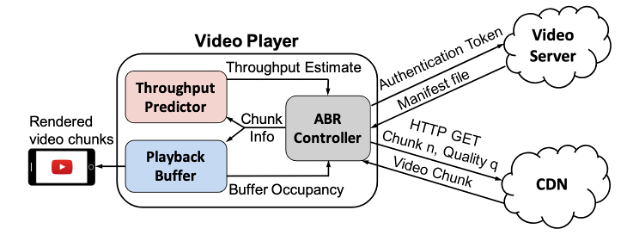
\includegraphics[width=\textwidth]{figures/chap02/abrteaser.png} 
                    \caption{自适应码率任务\cite{mao2017neural}}
                \end{subfigure}%
                \hfill
                \begin{subfigure}{0.49\textwidth}
                    \centering
                    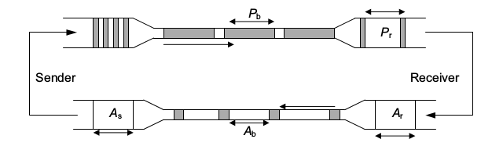
\includegraphics[width=\textwidth]{figures/chap02/sending.png} 
                    \caption{拥塞控制任务\cite{author2024performance}}
                \end{subfigure}
                \vspace{-1em}
                \caption{传输速率控制策略的工作形式}

            \end{figure}
            
\end{frame}


\begin{frame}[fragile]{研究背景}
\framesubtitle{发展趋势}
    \begin{itemize}
        \item 趋势:\textbf{应用传输需求的异质性}增加和\textbf{策略环境适配的差异性}增大。
    \end{itemize}
    \begin{columns}
        \begin{column}{0.6\textwidth}
            \begin{colorblock}[black]{sinteflightgreen}{}
            应用传输需求的异质性增加的原因:应用场景增多,服务目标和用户偏好分化
            \begin{equation}
                \scriptsize
                \begin{aligned}
                    QoE = \sum_{n=1}^{N}q(R_n) - \mu \sum_{n=1}^{N}q(T_n) - \sum_{n=1}^{N-1}\lvert q(R_{n+1})-q(R_n) \rvert.
                \end{aligned}
                \label{equation-qoe}
            \end{equation}
            \begin{table}[ht]
\centering
\resizebox{0.8\columnwidth}{!}{%
\begin{tabular}{@{}ccc@{}}
\toprule
\textbf{配置} & \textbf{码率利用率 (q(R))} & \textbf{Rebuffer 惩罚 ($\mu$)} \\
\midrule
$QoE_{\text{lin}}$  & R & 4.3 \\
$QoE_{\text{log}}$ & $\log\left(\frac{R}{R_{\text{min}}}\right)$ & 2.66 \\
$QoE_{\text{hd}}$ & 0.3 $\to$ 1, 0.7 $\to$ 2, \dots & 8 \\
\bottomrule
\end{tabular}
}
\label{table:bitrate-utility}
\end{table}

            \end{colorblock}
            
        \end{column}

        \begin{column}{0.45\textwidth}
        
            \begin{block}{}
              策略环境适配的差异性增大的原因:网络介质更新和使用率增加,网络更波动,策略需适应的环境更多变,如高铁上网络、无线网络、高时延网络。
            \begin{figure} [ht]
            \centering
            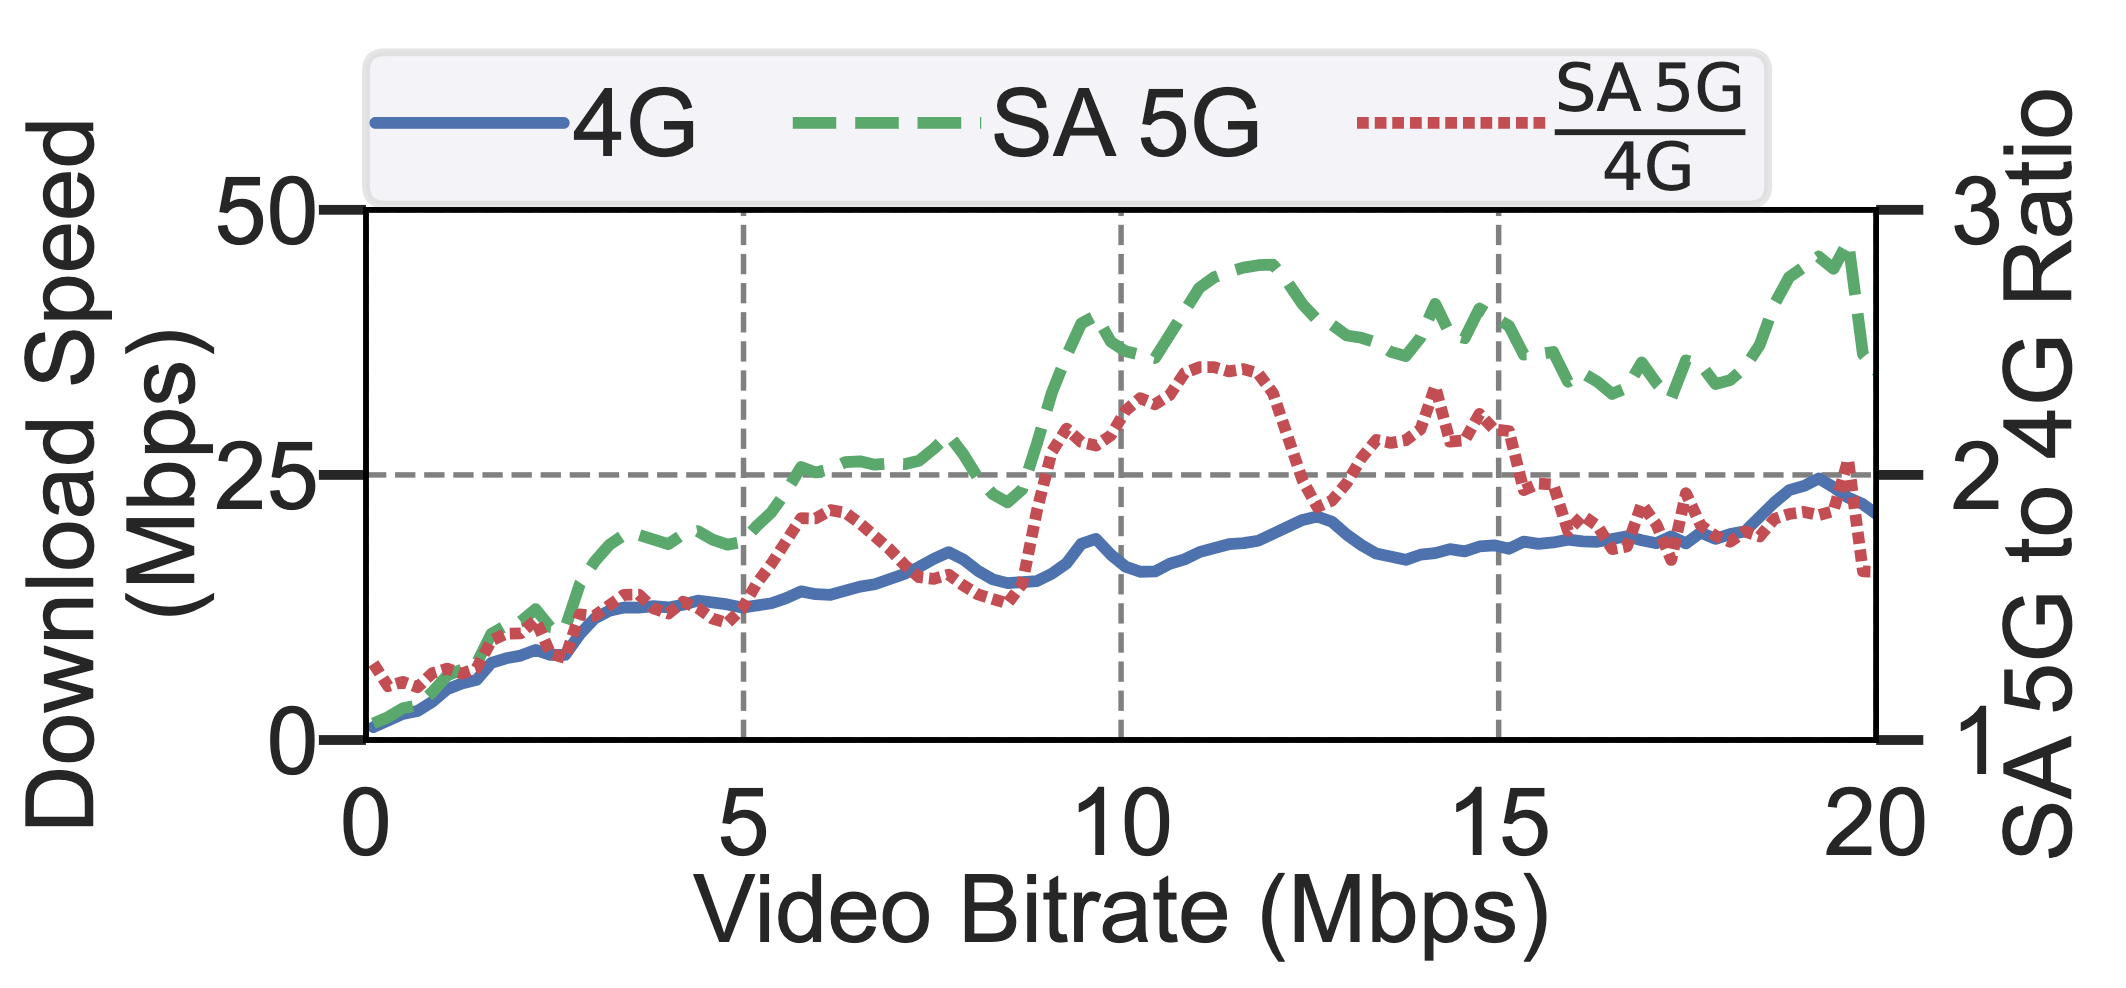
\includegraphics[width=0.6\textwidth]{figures/applications/趋势.png} 
            \caption{差异化的网络环境\cite{10.1145/3544216.3544219}}
            \end{figure}
            
            \end{block}
              
        \end{column}

    \end{columns}

\end{frame}


% \begin{frame}[fragile]{研究背景}
% \framesubtitle{发展趋势}
%     \begin{itemize}
%         \item 趋势:\textbf{应用传输需求的异质性}增加和\textbf{策略环境适配的差异性}增大。
%     \end{itemize}
%     \begin{columns}
%         \begin{column}{0.5\textwidth}
%             \begin{colorblock}[black]{sinteflightgreen}{}
%             应用传输需求的异质性增加的原因:应用场景增多,服务目标和用户偏好分化
%                 \begin{figure}[ht]
\centering
\begin{subfigure}[t]{0.48\linewidth} 
  \centering
  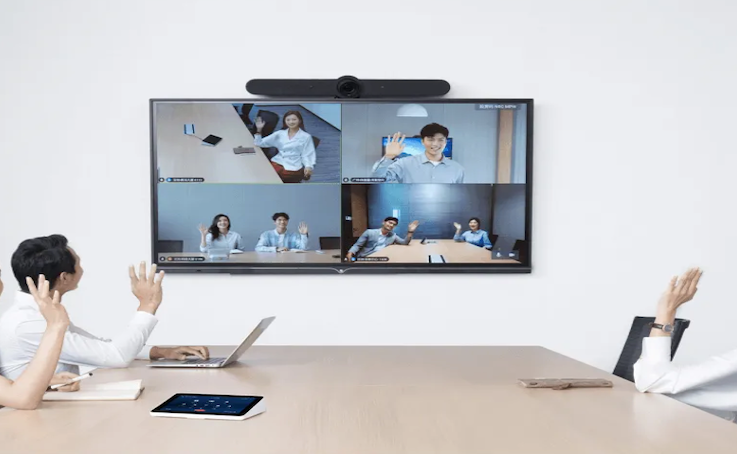
\includegraphics[height=0.2\textheight]{figures/applications/meet.png} % 设置图像高度
  \caption{视频会议}
\end{subfigure}%
\begin{subfigure}[t]{0.48\linewidth} 
  \centering
  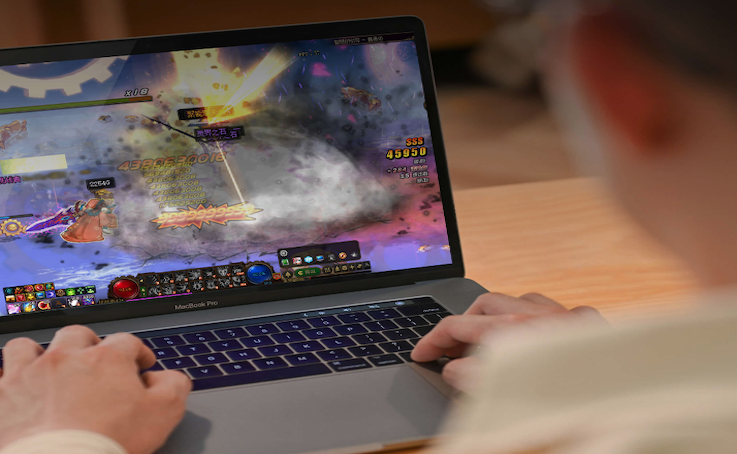
\includegraphics[height=0.2\textheight]{figures/applications/cloudgame.png} % 设置图像高度
  \caption{云游戏}
\end{subfigure}

\vspace{-0.5em} 
\begin{subfigure}[t]{0.48\linewidth} 
  \centering
  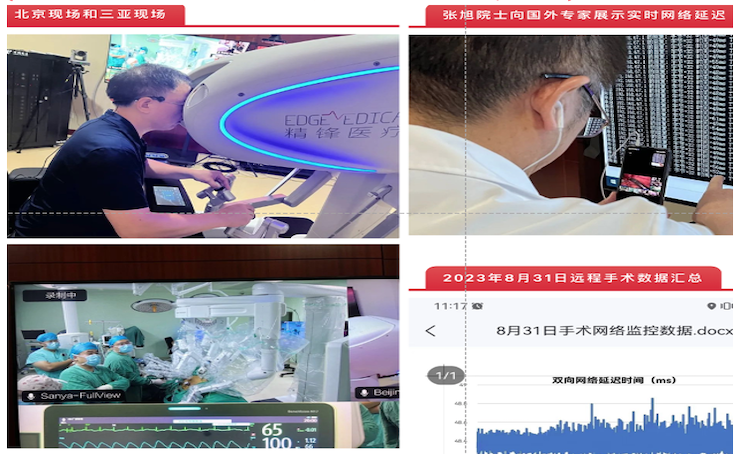
\includegraphics[height=0.2\textheight]{figures/applications/surgury.png} % 设置图像高度
  \caption{远程手术}
\end{subfigure}%
\begin{subfigure}[t]{0.48\linewidth} 
  \centering
  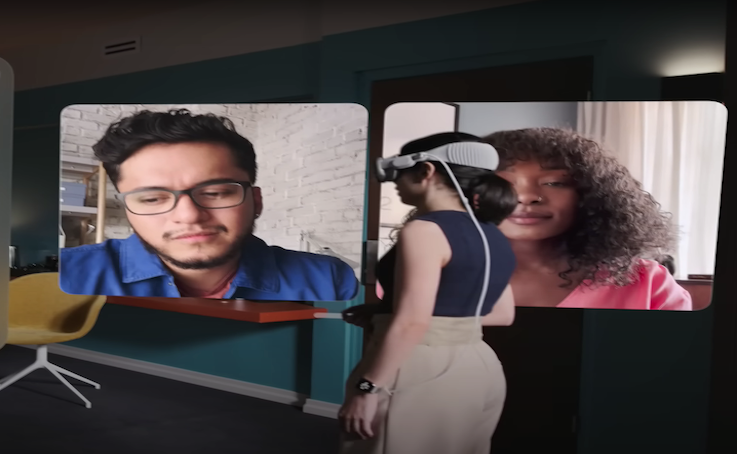
\includegraphics[height=0.2\textheight]{figures/applications/vr.png} % 设置图像高度
  \caption{VR应用}
  \label{fig-chess-game}
\end{subfigure}
\vspace{-1em} % 减小间距
\caption{传输速率控制策略的使用场景}
\label{fig-apps}
\end{figure}

%             \end{colorblock}
            
%         \end{column}

%         \begin{column}{0.5\textwidth}
        
%             \begin{block}{}
%               策略环境适配的差异性增大的原因:网络介质更新和使用率增加,网络更波动,策略需适应的环境更多变,如高铁上网络、无线网络、高时延网络。
%             \begin{figure} [ht]
%             \centering
%             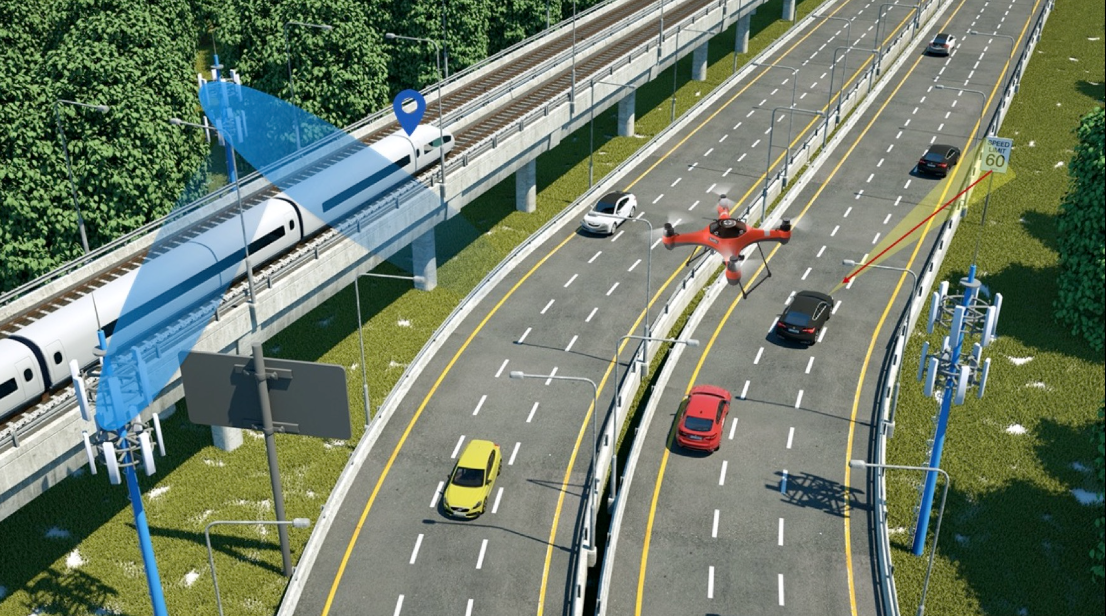
\includegraphics[width=0.6\textwidth]{figures/applications/截屏2024-12-01 19.44.49.png} 
%             \caption{差异化的网络环境}
%             \end{figure}
            
%             \end{block}
              
%         \end{column}

%     \end{columns}

% \end{frame}


\begin{frame}[fragile]{研究问题}
\framesubtitle{问题的引入}
        \begin{figure} [ht]
        \centering
        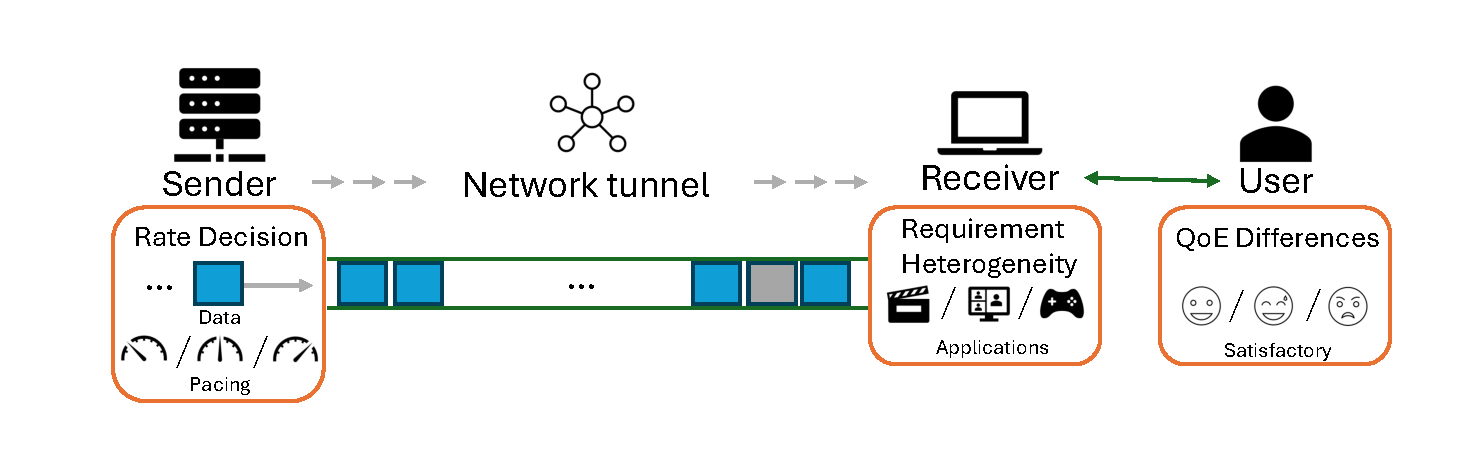
\includegraphics[width=0.7\textwidth]{figures/chap01/system_archi.pdf} 
        \caption{网络传输速率控制的系统架构}
        \label{fig:teaser_system_archi}
        \end{figure} 
    
        \begin{itemize}
        \item 当下的控制模块(1)缺乏对场景的感知能力和差异化控制策略;(2)工作范式对不同网络环境特性采用固定的策略选择,造成了服务质量的次优。
        \item \alert{能否设计能感知场景偏好的策略,及利用现存策略库来提升服务质量?}
    \end{itemize}
\end{frame}

\begin{frame}[fragile]{研究挑战与内容}
\framesubtitle{解决问题面临的挑战、内容与目标}

    \begin{columns}
        \begin{column}{0.35\textwidth}
            \begin{colorblock}[black]{sinteflightgreen}{}
            \begin{itemize}
                \item 挑战1: 根据QoE确定策略优化目标
                \item 挑战2: 根据优化目标设计传输速率控制算法
                \item 挑战3: 利用累积策略库构建控制范式
                
            \end{itemize}
            \end{colorblock}
            
        \end{column}

        \begin{column}{0.72\textwidth}
            \begin{figure} [ht]
            \centering
            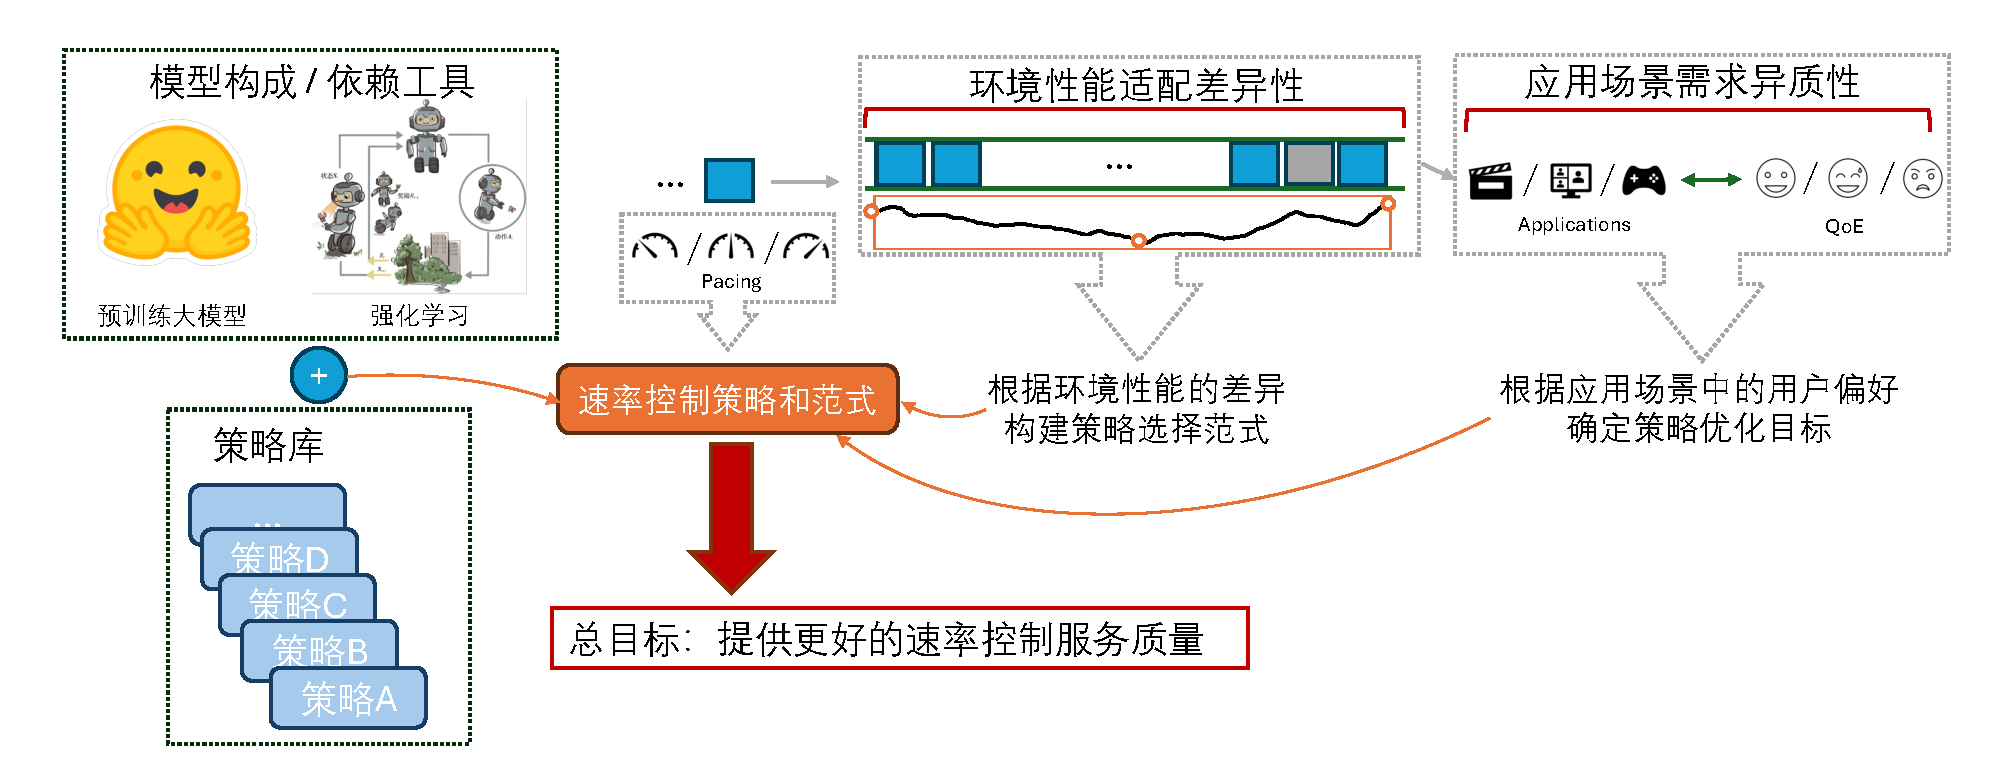
\includegraphics[width=\textwidth]{figures/chap01/final_goal.pdf} 
            \caption{研究内容}
            \label{fig:teaser_system_archi}
            \end{figure} 
        \vspace{-2em}
        
        \end{column}
        
    \end{columns}

    \begin{block}{}
            \begin{itemize}
                \item 研究目标1: 设计可对场景中用户偏好感知的云游戏实时通信传输速率控制算法
                \item 研究目标2: 重构累积策略库构建可动态变化策略的控制范式
            \end{itemize}            
        \end{block}
\end{frame}

\begin{frame}[fragile]{论文组织架构}
\framesubtitle{各章内容安排与逻辑关系}
    \begin{figure} [ht]
    \centering
    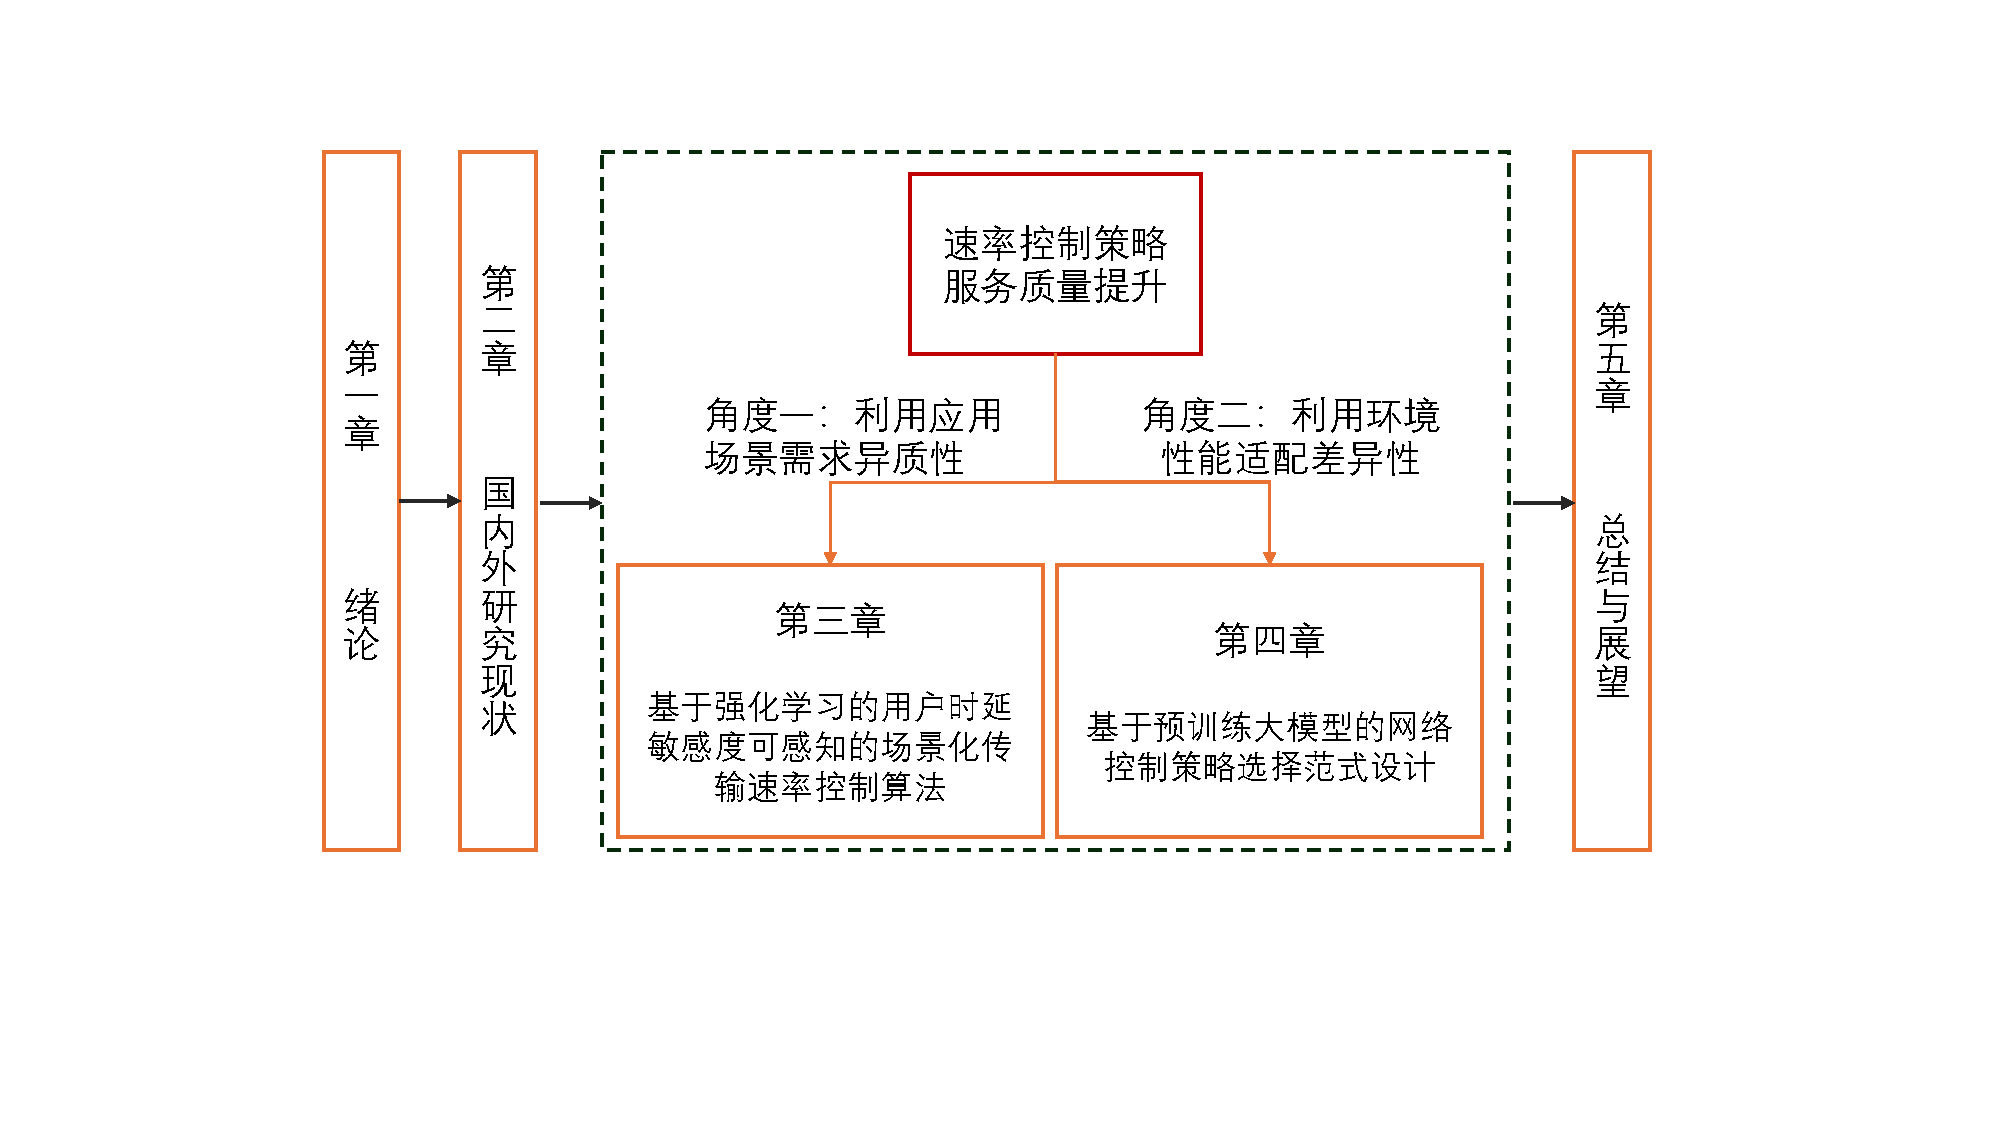
\includegraphics[width=0.75\textwidth]{figures/chap01/arrange.pdf} 
    \caption{本文各章内容安排与结构}
    \label{fig:arrange}
    \end{figure}

\end{frame}

\section{国内外研究现状}

\begin{frame}[fragile]{国内外研究现状}
\framesubtitle{框架组织}
    \begin{figure} [ht]
    \centering
    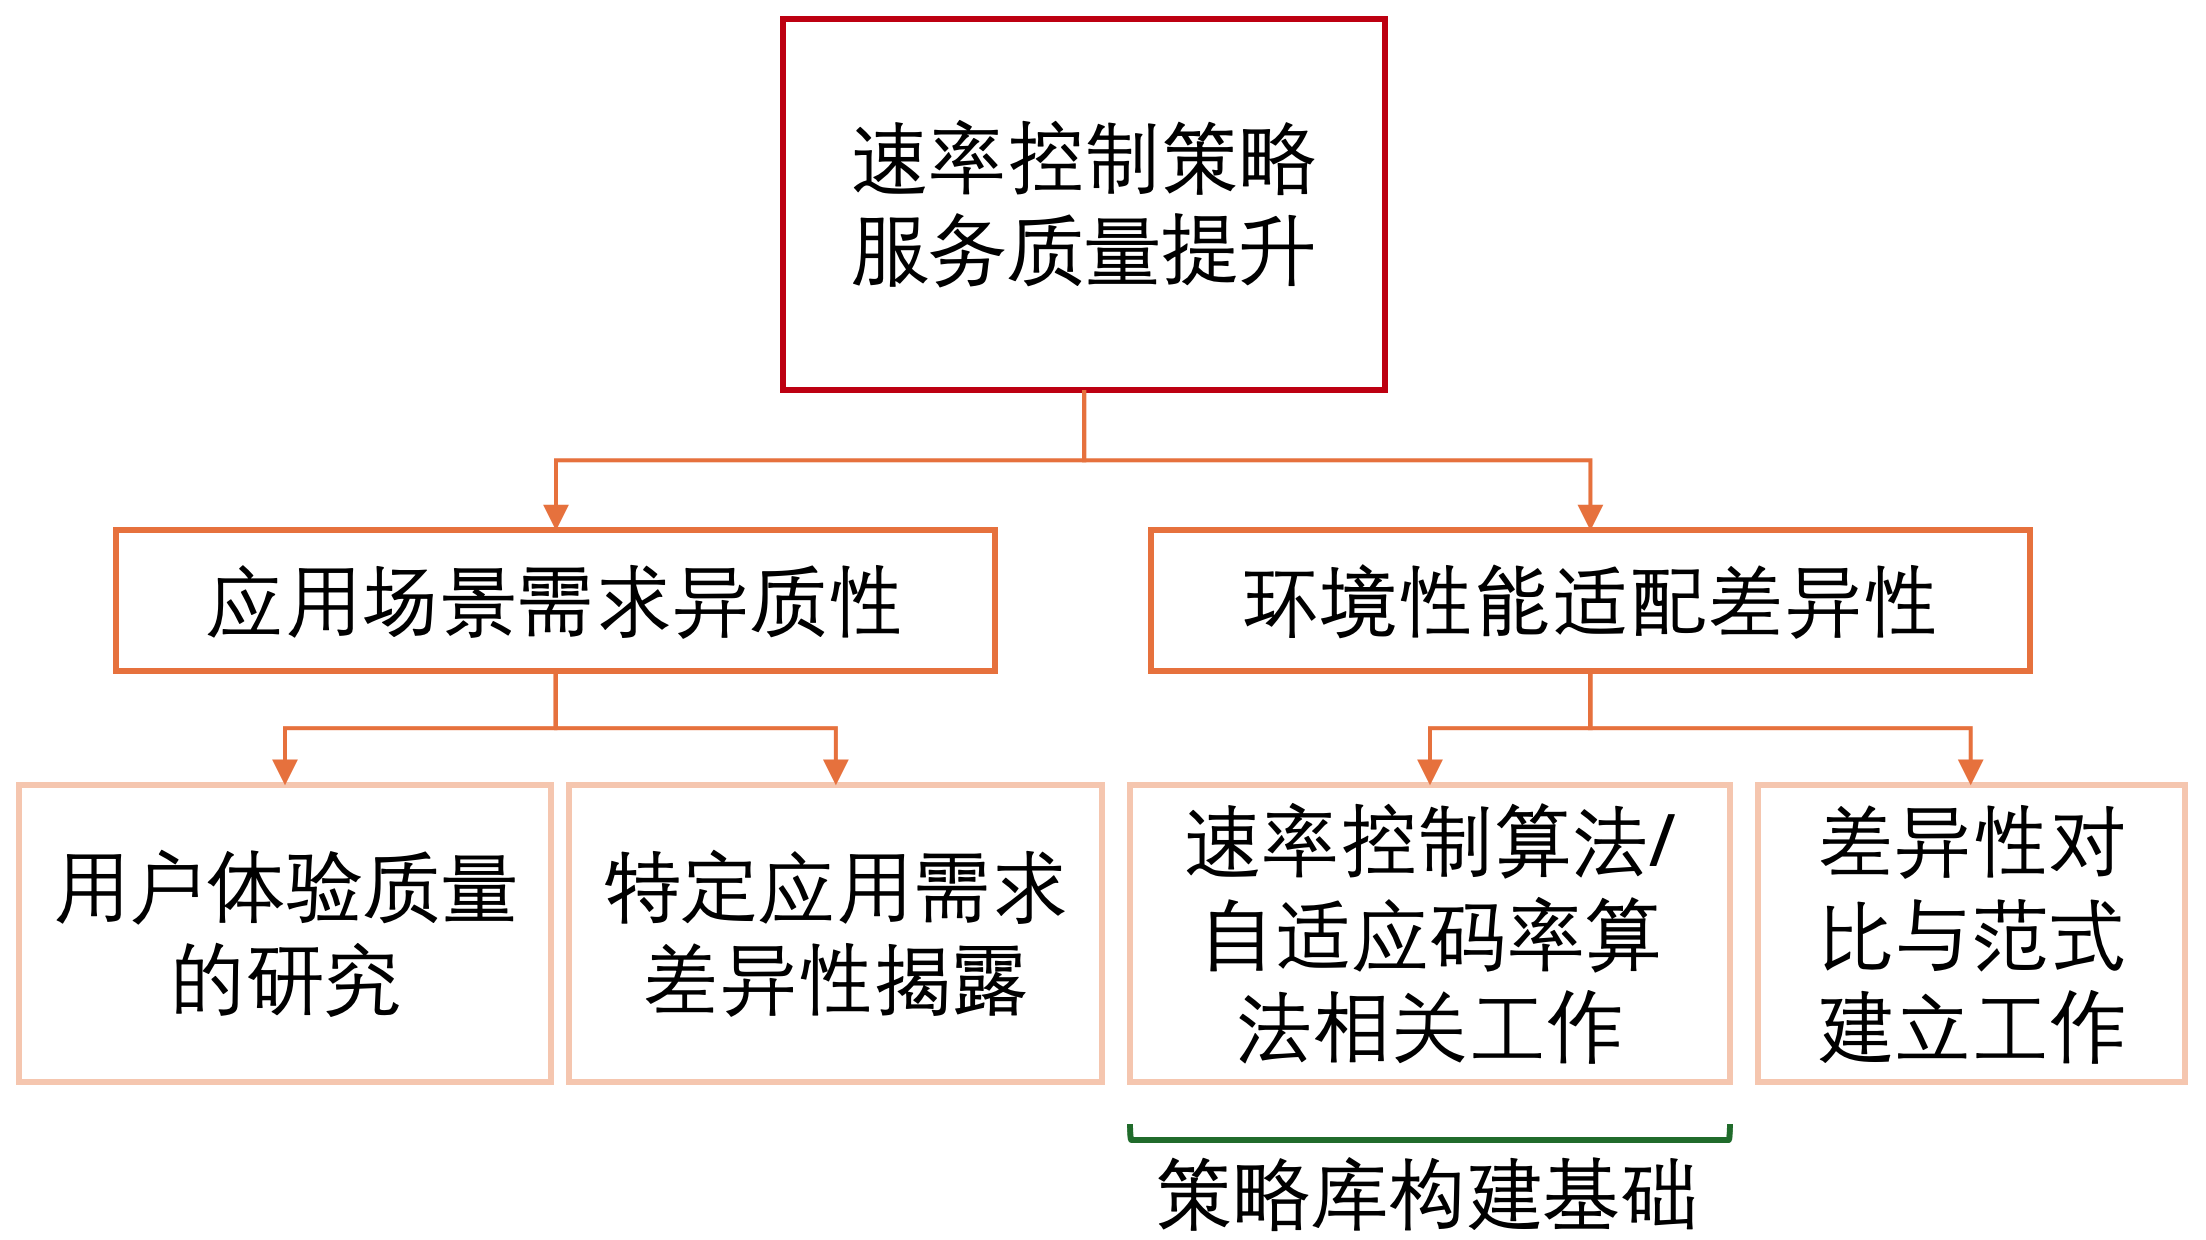
\includegraphics[width=0.75\textwidth]{figures/chap02/related.png} 
    \caption{国内外研究现状的组成与结构}
    \label{fig:arrange}
    \end{figure}
\end{frame}

\begin{frame}[fragile]{国内外研究现状}
\framesubtitle{应用场景需求异质性的研究}
    \begin{columns}
        \begin{column}{0.55\textwidth}
            \begin{colorblock}[black]{sintefyellow}{}
            \begin{figure}[ht]
\centering
\begin{subfigure}[t]{0.48\linewidth} 
  \centering
  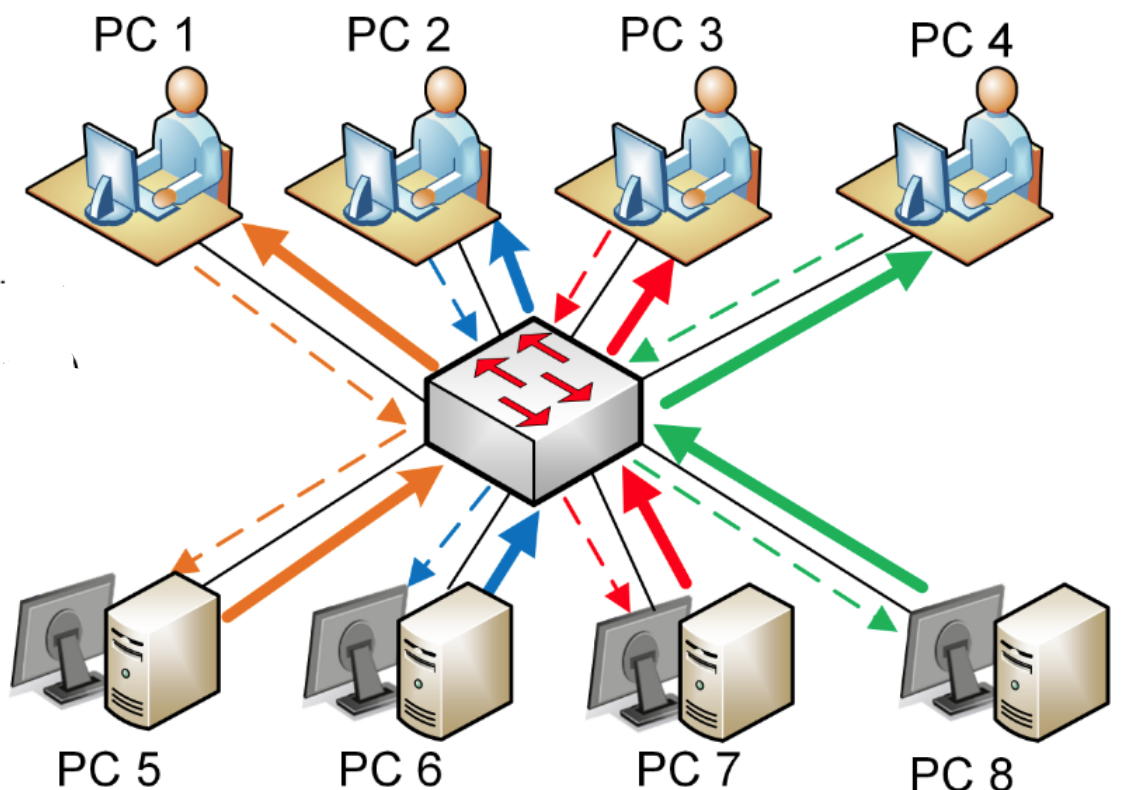
\includegraphics[height=0.2\textheight]{figures/chap02/qoe_related/MOS.png} % 设置图像高度
  \caption{MOS实验}
\end{subfigure}%
\begin{subfigure}[t]{0.48\linewidth} 
  \centering
  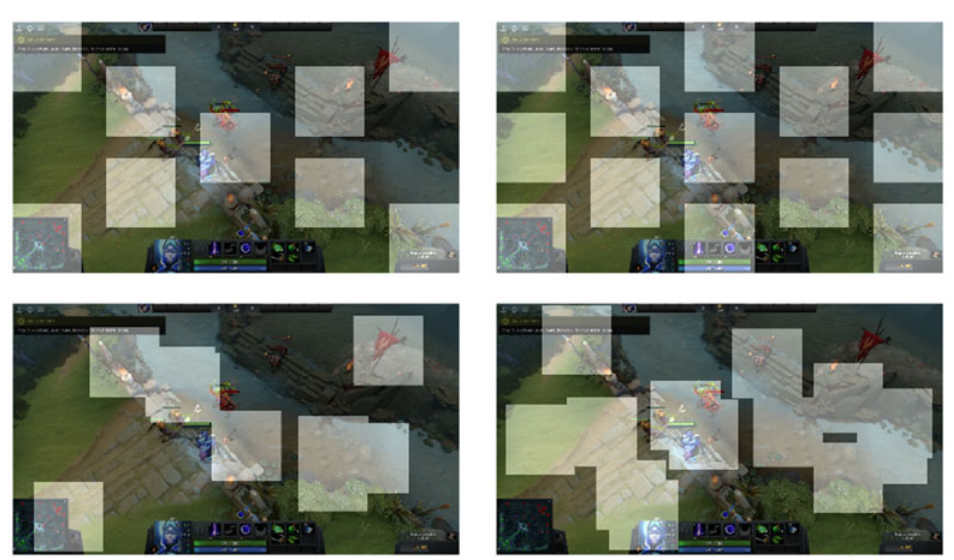
\includegraphics[height=0.2\textheight]{figures/chap02/qoe_related/VMAF.png} % 设置图像高度
  \caption{画面评价}
\end{subfigure}

\vspace{-0.5em} 
\begin{subfigure}[t]{0.48\linewidth} 
  \centering
  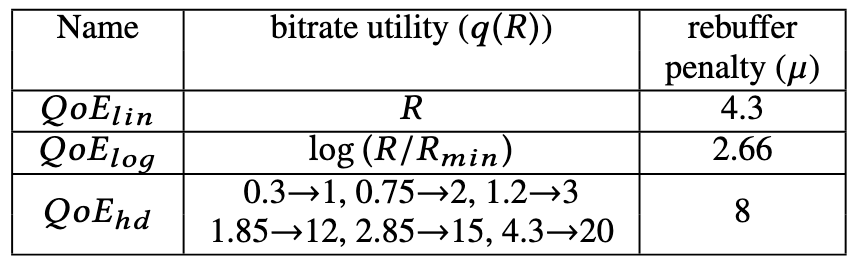
\includegraphics[height=0.2\textheight]{figures/chap02/qoe_related/QoS代替QoE.png} % 设置图像高度
  \caption{QoS指标计算QoE}
\end{subfigure}%
\begin{subfigure}[t]{0.48\linewidth} 
  \centering
  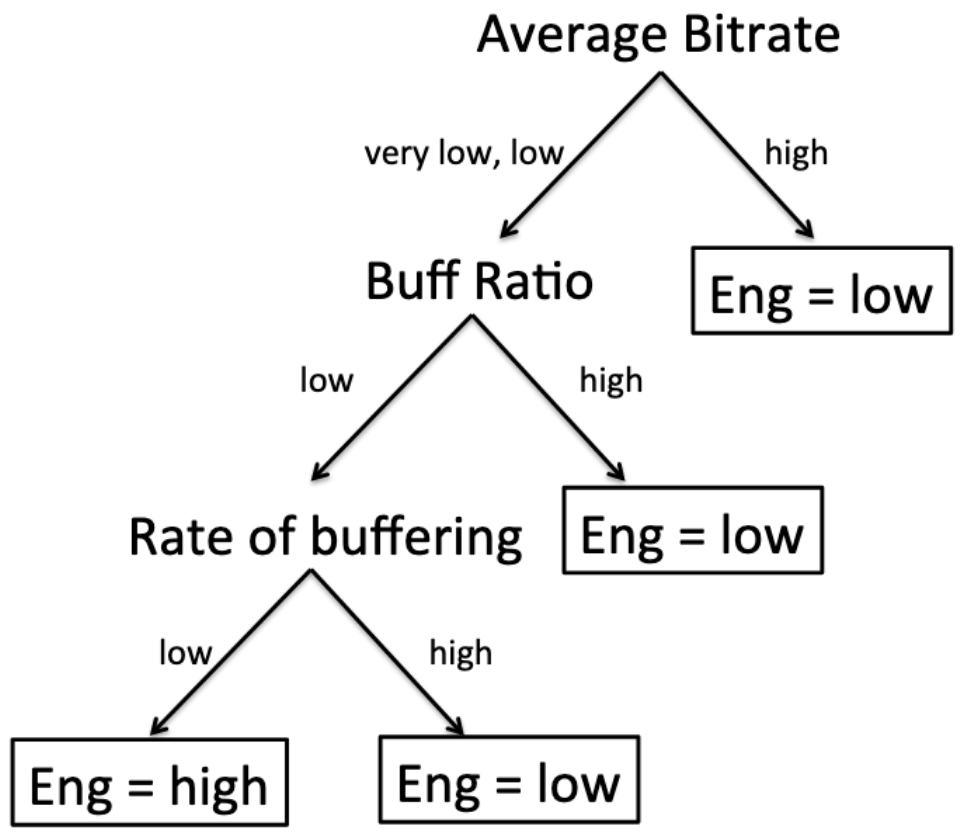
\includegraphics[height=0.2\textheight]{figures/chap02/qoe_related/model.png} % 设置图像高度
  \caption{主客观模型预测}
  \label{fig-chess-game}
\end{subfigure}
\vspace{-1em} % 减小间距
\caption{用户体验质量研究}
\label{fig-qoe-re}
\end{figure}

            \end{colorblock}

        \end{column}
    
        \begin{column}{0.45\textwidth}
        \begin{block}{场景需求差异性揭露}
            \begin{itemize}
                \item ClayPool:网络游戏中玩家对于操作响应和画面变化延迟的敏感性\cite{claypool2006latency,claypool2010latency}

                \item EyeQoE\cite{zhu2022eyeqoe}:360$^{\circ}$视频的播放对用户的眼球运动分类并捕捉运动模式
                \item Michael:游戏节奏的差异性\cite{jarschel2011evaluation}
                \item ...
            \end{itemize}
        
        \end{block}

        \end{column}
    \end{columns}
    \vspace{0.3em}
    \alert{工作的问题:止步于用户研究/差异性,而未直接用于策略设计或联合其特性。}

\end{frame}

\begin{frame}[fragile]{国内外研究现状}
\framesubtitle{环境性能适配差异性的研究}
        \begin{columns}
        \begin{column}{0.58\textwidth}
            \begin{colorblock}[black]{sintefyellow}{}
            \begin{figure}[ht]
\centering
\begin{subfigure}[t]{0.49\linewidth}
  \centering
  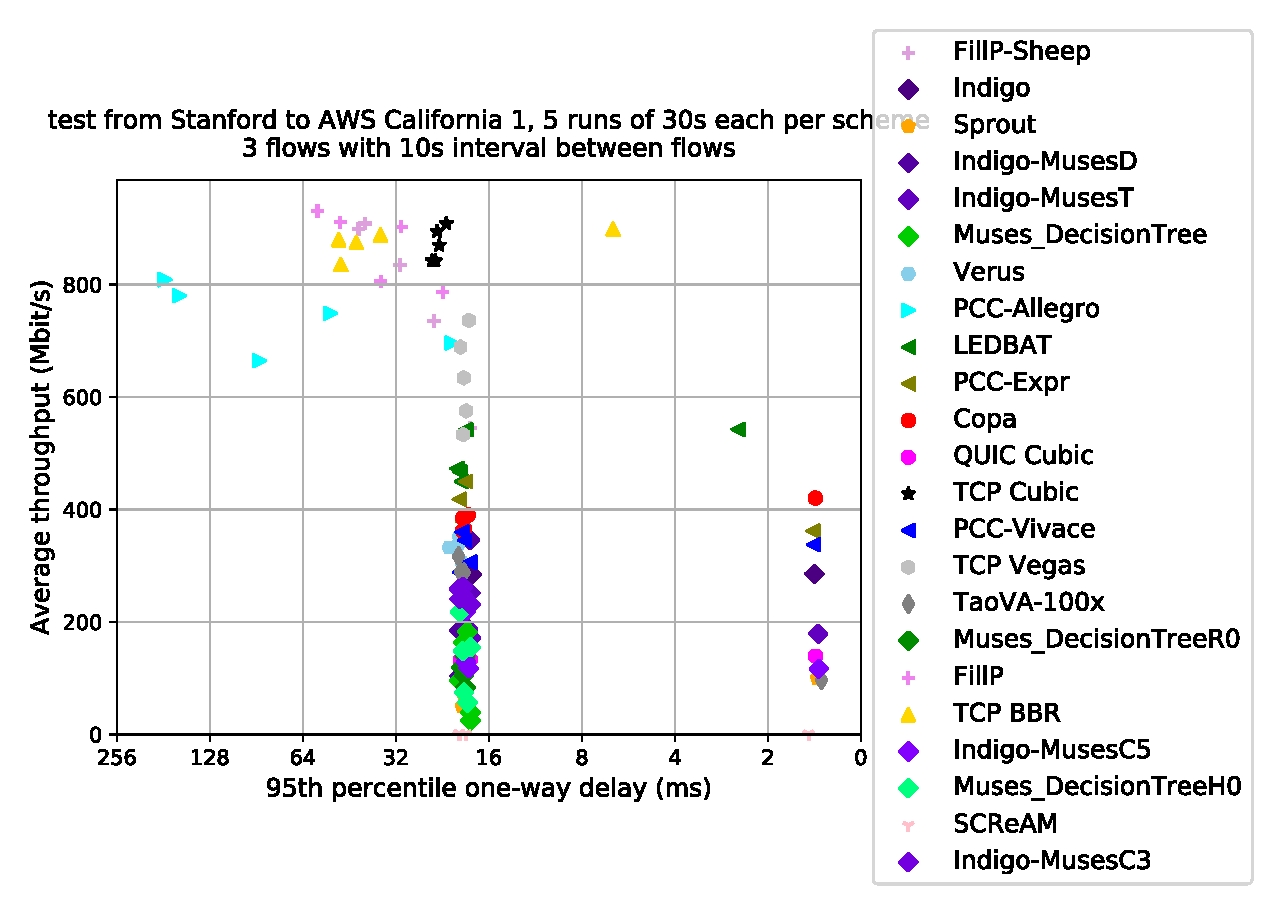
\includegraphics[width=\linewidth]{figures/chap02/measument-ccabr/cc.pdf}
  \caption{拥塞控制算法性能评测}
  \label{fig-measument-ccabr-cc}
\end{subfigure}%
\begin{subfigure}[t]{0.49\linewidth}
  \centering
  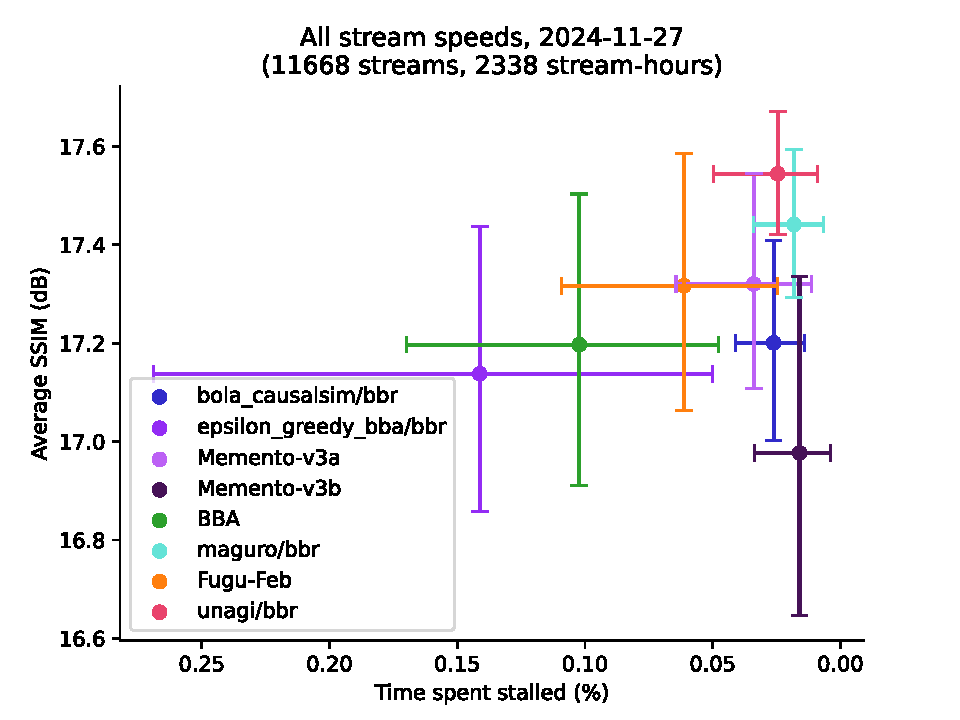
\includegraphics[width=\linewidth]{figures/chap02/measument-ccabr/abr.pdf}
  \caption{自适应码率算法性能评测}
  \label{fig-measument-ccabr-abr}
\end{subfigure}

\caption{Pantheon\cite{yan2018pantheon}和Puffer\cite{yan2020learning}的性能测量结果}
\label{fig-mea-ccabr}
\end{figure}

            \end{colorblock}
                    \alert{研究空白:尽管有大量速率控制策略,没有针对速率控制策略的选择范式。}
        \end{column}
    
        \begin{column}{0.44\textwidth}        \begin{block}{差异性对比与范式工作}
            \begin{itemize}
                \item NetLLM\cite{wu2024netllm}:用了一个多模态编码器对网络应用进行决策的范式

                \item LLM-ABR\cite{he2024llm}:让大模型生成出可用的ABR策略,并通过一系列检测和性能测试后使用,进而构建了一个策略创建范式。
                \item Sage\cite{yen2023computers}: 将过去几十年来的所有拥塞算法的工作模式和行为通过强化学习的方式迁移到它自身身上
                \item ...
            \end{itemize}

        \end{block}

        \end{column}
    \end{columns}
\end{frame}

\section{基于强化学习的用户时延敏感度可感知的场景化传输速率控制算法}

\begin{frame}[fragile]{基于强化学习的用户敏感度可感知的速率控制算法}
\framesubtitle{算法设计概览}

\begin{figure}[ht]
    \centering
    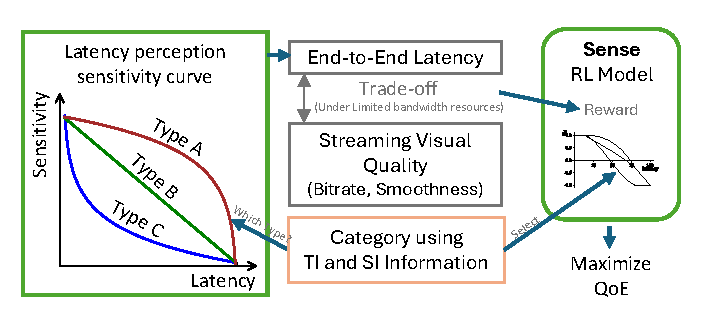
\includegraphics[width=0.55\textwidth]{figures/chap03/teaser.pdf}
    \caption{敏感度可感知的云游戏传输速率控制算法的设计框架}
    \label{fig:teaser}
\end{figure}
\begin{colorblock}[black]{sinteflightgreen}{}
\begin{itemize}
    \item 在有限带宽条件下,端到端时延和视觉质量之间的权衡对用户体验有显著影响。
    \item 工作根据主客观实验确定的延迟感知敏感度曲线做出发送速率的权衡;
    \item 使用画面信息进行场景分类,并对不同的场景采取差异化的发送策略
\end{itemize}
            \end{colorblock}
\end{frame}

\begin{frame}[fragile]{基于强化学习的用户敏感度可感知的速率控制算法}
\framesubtitle{客观测量实验和动机}

            \begin{figure}[htbp]
\centering
\begin{subfigure}[t]{0.33\linewidth}
  \centering
  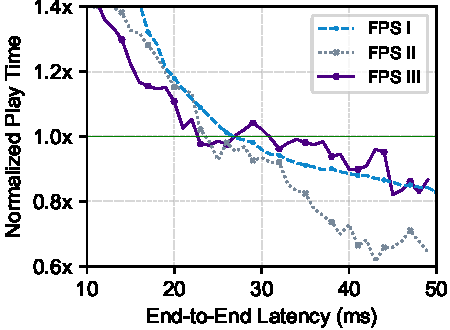
\includegraphics[width=\linewidth]{figures/chap03/measurement_data/delay-sensitive.pdf}
  \caption{高敏感度游戏}
  \label{fig-real-measurement-results-High-Delay-Sensitivity-Games}
\end{subfigure}%
\begin{subfigure}[t]{0.33\linewidth}
  \centering
  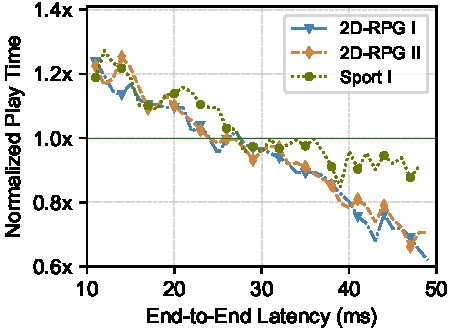
\includegraphics[width=\linewidth]{figures/chap03/measurement_data/delay-linear-sensitive.pdf}
  \caption{中敏感度游戏}
  \label{fig-real-measurement-Medium-Delay-Sensitivity-Games}
\end{subfigure}
\begin{subfigure}[t]{0.33\linewidth}
  \centering
  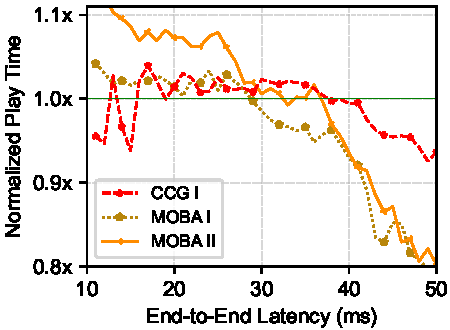
\includegraphics[width=\linewidth]{figures/chap03/measurement_data/delay-not-sensitive.pdf}
  \caption{低敏感度游戏}
  \label{fig-real-measurement-results-Low-Delay-Sensitivity-Games}
\end{subfigure}%
\label{fig:measurement-result}
\end{figure}


            \begin{colorblock}[black]{sinteflightgreen}{}
            \begin{itemize}
            \item 借助腾讯平台展开大规模数据测量以确定不同游戏场景的表现差异;
            \item 使用时长与时延变化的趋势可被归类为三类。
        \end{itemize}
            \end{colorblock}
\end{frame}




\begin{frame}[fragile]{基于强化学习的用户敏感度可感知的速率控制算法}
\framesubtitle{主观实验和动机}
    \begin{columns}
        \begin{column}{0.65\textwidth}
                \begin{figure}[ht]
\centering
\begin{subfigure}[t]{0.5\linewidth}
  \centering
  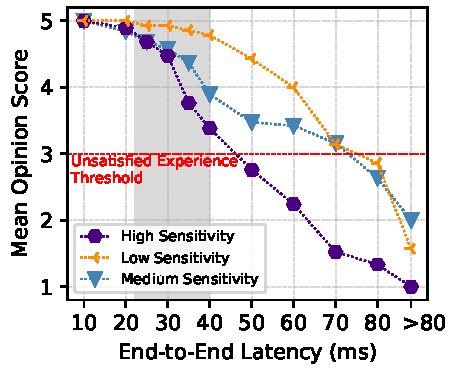
\includegraphics[width=\linewidth]{figures/chap03/latency_curve/user_perception.pdf}
  \caption{用户平均MOS评分}
  \label{fig-average-user-mos-rating}
\end{subfigure}%
\begin{subfigure}[t]{0.5\linewidth}
  \centering
  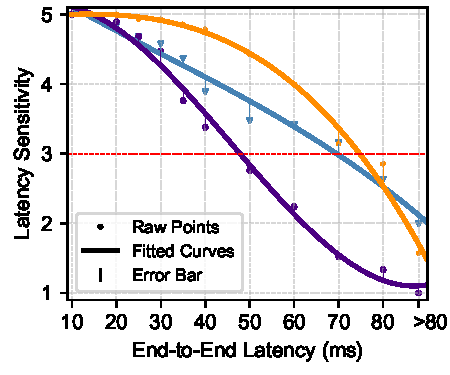
\includegraphics[width=\linewidth]{figures/chap03/latency_curve/fitted_curve.pdf}
  \caption{拟合曲线}
  \label{fig-fitted-curves}
\end{subfigure}
\caption{用户MOS评分实验结果和数值拟合结果}
\label{fig-latency-curve}
\end{figure}

        \end{column}

        \begin{column}{0.35\textwidth}             
            \begin{colorblock}[black]{sinteflightgreen}{}
                \begin{itemize}
                    \item 基于分类展开不同时延下用户满意度打分实验;
                    \item 将实验结果通过最小二乘法拟合为“敏感度”量化指标。
                \end{itemize}
            \end{colorblock}
        \end{column}
    \end{columns}



\end{frame}


\begin{frame}[fragile]{基于强化学习的用户敏感度可感知的速率控制算法}
\framesubtitle{强化学习算法设计}


        \begin{columns}
\begin{column}{0.48\textwidth}
\begin{block}
\small  % 将字体大小设置为较小
\begin{figure}[ht]
\centering
\begin{subfigure}[t]{0.4\linewidth}
  \centering
  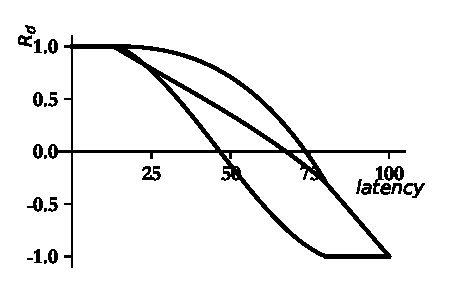
\includegraphics[width=\linewidth]{figures/chap03/reward_function/Rd.pdf}
  \caption{延迟奖励}
  \label{fig:Latency Reward}
\end{subfigure}%
\hspace{0.05\linewidth} % 添加水平间距
\begin{subfigure}[t]{0.4\linewidth}
  \centering
  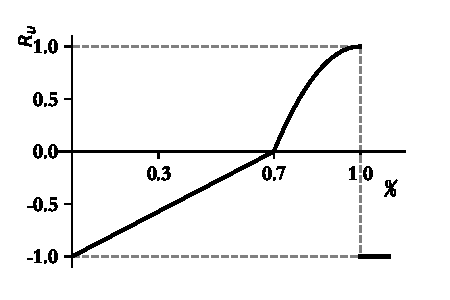
\includegraphics[width=\linewidth]{figures/chap03/reward_function/Ru.pdf}
  \caption{带宽利用率奖励}
  \label{fig:Bandwidth Utilization Reward}
\end{subfigure}

\vspace{0.5em} % 适当增加垂直间距
\begin{subfigure}[t]{0.4\linewidth}
  \centering
  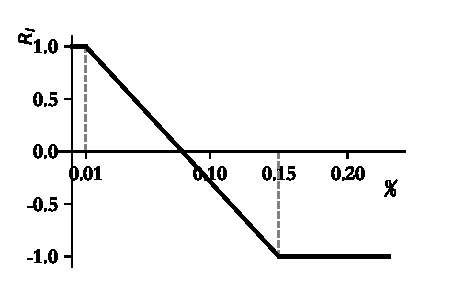
\includegraphics[width=\linewidth]{figures/chap03/reward_function/Rl.pdf}
  \caption{丢包率奖励}
  \label{fig:Loss Ratio Reward}
\end{subfigure}%
\hspace{0.05\linewidth} % 添加水平间距
\begin{subfigure}[t]{0.4\linewidth}
  \centering
  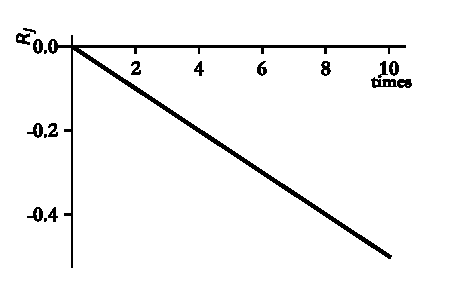
\includegraphics[width=\linewidth]{figures/chap03/reward_function/Rj.pdf}
  \caption{屏幕抖动奖励}
  \label{fig:jitter Reward}
\end{subfigure}

\caption{强化学习中的奖励函数构成}
\label{fig:reward-function}
\end{figure}

\end{block}
\end{column}

\begin{column}{0.5\textwidth}
\begin{colorblock}[black]{sinteflightgreen}{强化学习空间的构成}
\begin{itemize}
    \scriptsize % 更小的字体
    \item 动作空间:发送速率 $R_s \in $[3, 50]$ Mbps$ 
    \begin{equation}
        \scriptsize % 更小的公式字体大小
        \begin{aligned}
            R_{slog} = \frac{\log(R_s)-\log(R_{min})}{\log(R_{max})-\log(R_{min})}.
        \end{aligned}
        \label{eq:logsend}
    \end{equation} 
    \item 状态空间:接收速率 $RR$;(ii)延迟 $D$;(iii)丢包率 $L$;(iv)帧间到达时间 $J$;(v)上一步动作 $a$
    \begin{equation}
        \scriptsize
        \begin{aligned}
        \mathcal{S}_t &= \left( \boldsymbol{s_t}, \boldsymbol{s_{t-1}}, \dots, \boldsymbol{s_{t-4}} \right), \\
        \boldsymbol{s_t} &= \left( RR_t, D_t, L_t, J_t, a_t \right)
        \end{aligned}
    \end{equation}
    \item 奖励空间: $\alpha_1, \alpha_2, \alpha_3, \alpha_4$超参;\begin{equation}
    \scriptsize
    \begin{aligned}
    R = \alpha_1 R_d + \alpha_2 R_u + \alpha_3 R_l + \alpha_4 R_j
    \end{aligned}
    \label{eq:total_reward}
    \end{equation}
\end{itemize}
\end{colorblock}

\end{column}

    \end{columns}
\end{frame}


\begin{frame}[fragile]{基于强化学习的用户敏感度可感知的速率控制算法}
\framesubtitle{场景分类方法}
\begin{columns}
    \begin{column}{0.5\textwidth}
        \begin{figure} [ht]
                \centering
                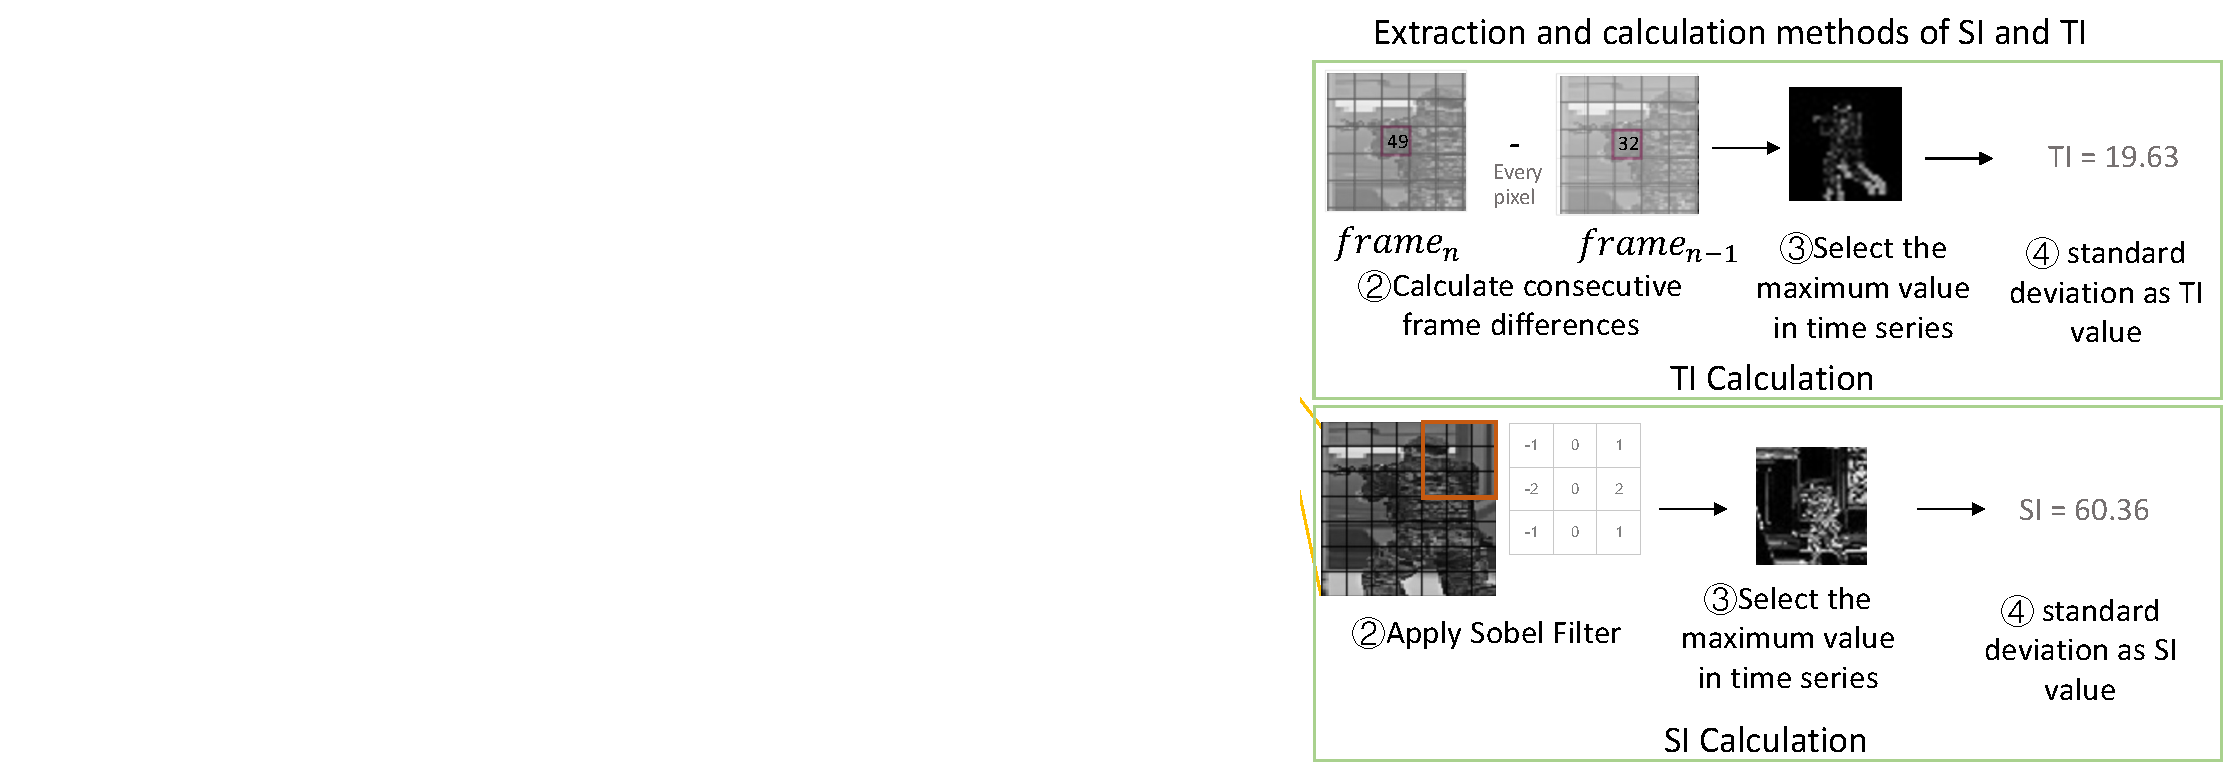
\includegraphics[width=\textwidth]{figures/chap03/intra_schematic_diagram.pdf} 
                \caption{两款游戏的TI和SI提取结果预览}
                \label{fig_intra_schematic_diagram}
                \end{figure}  
    \end{column}

    \begin{column}{0.5\textwidth}
        \begin{table}[ht]
\centering
\caption{游戏的 SI 和 TI 使用 K-Means 方法进行分类的结果,准确率:89.4\%}
\resizebox{0.66\columnwidth}{!}{%
\begin{tabular}{@{}ccccc@{}}
\toprule
游戏 & TI & SI & K-means分类 & 正确分类 \\ \midrule
3D-RPG I           & 8.10  & 48.73  & 高敏感度          & 是                    \\
TPS I              & 18.42 & 55.39  & 高敏感度          & 是                    \\
\textbf{FPS III}   & 18.22 & 67.94  & 高敏感度          & 是                    \\
FPS IV             & 17.69 & 71.55  & 高敏感度          & 是                    \\
\textbf{FPS II}    & 16.55 & 72.05  & 高敏感度          & 是                    \\
\textbf{CCG I}     & 2.12  & 74.63  & 低敏感度           & 是                    \\
Sport III          & 11.29 & 77.00  & 低敏感度           & 否 (中敏感度)                   \\
3D-RPG II          & 10.31 & 80.21  & 低敏感度           & 是                    \\
A-RPG I            & 4.03  & 81.97  & 低敏感度           & 是                    \\
MMORPG II          & 14.02 & 84.21  & 低敏感度           & 是                    \\
MMORPG I           & 21.34 & 86.12  & 低敏感度           & 是                    \\
\textbf{MOBA I}    & 3.40  & 87.00  & 低敏感度           & 是                    \\
\textbf{MOBA II}   & 3.74  & 87.51  & 低敏感度           & 是                    \\
FPS I              & 27.74 & 89.25  & 低敏感度           & 否 (高敏感度)
                        \\
Casual III         & 10.73 & 91.49  & 中敏感度          & 是                    \\
Casual II          & 8.39  & 92.64  & 中敏感度          & 是                    \\
\textbf{Sport I}   & 11.76 & 103.32 & 中敏感度          & 是                    \\
\textbf{2D-RPG I}  & 8.13  & 108.18 & 中敏感度          & 是                    \\
\textbf{2D-RPG II} & 17.33 & 119.28 & 中敏感度          & 是                    \\ \bottomrule
\end{tabular}
}
\label{tab_cat_gor}
\end{table}
        
    \end{column}
\end{columns}



                

\end{frame}
\begin{frame}[fragile]{基于强化学习的用户敏感度可感知的速率控制算法}
\framesubtitle{评估与实验结果}
        \begin{columns}
            \begin{column}{0.45\textwidth}
            \begin{block}{}
\begin{figure}[ht]
\centering
\begin{subfigure}[t]{0.4\linewidth}
  \centering
  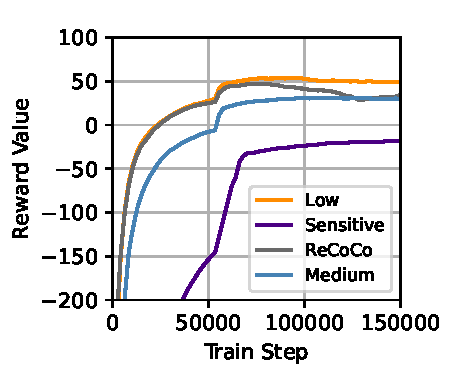
\includegraphics[width=\linewidth]{figures/chap03/evaluation_plots/reward_value.pdf}
  \caption{训练奖励累计}
  \label{fig-reward-func}
\end{subfigure}%
\hspace{0.02\linewidth} % 调整左右图之间的间距
\begin{subfigure}[t]{0.4\linewidth}
  \centering
  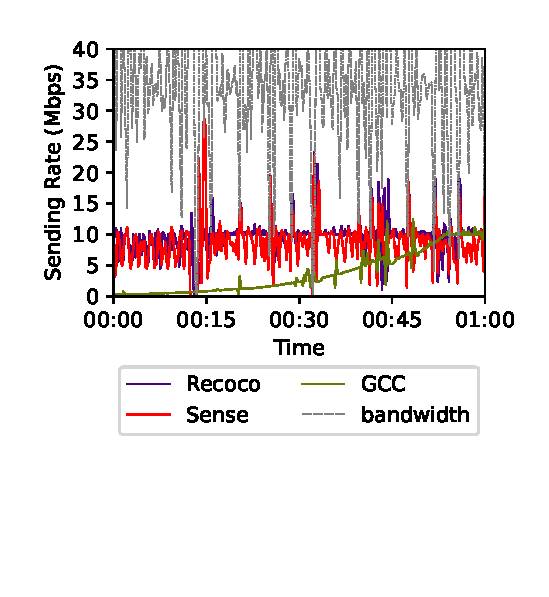
\includegraphics[width=\linewidth]{figures/chap03/evaluation_plots/bandwidth.pdf}
  \caption{带宽利用率}
  \label{fig-band-util}
\end{subfigure}

\vspace{-0.1cm} % 减少图形之间的垂直间距

\begin{subfigure}[t]{0.4\linewidth}
  \centering
  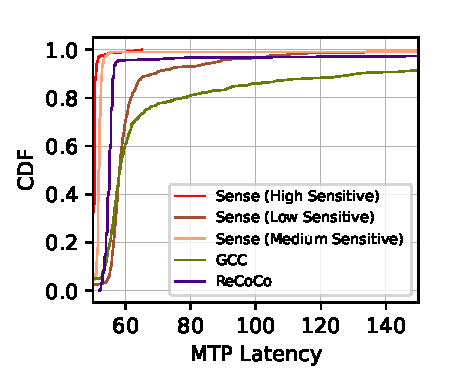
\includegraphics[width=\linewidth]{figures/chap03/evaluation_plots/cdf_delay.pdf}
  \caption{延迟CDF}
  \label{fig-latency-cdf}
\end{subfigure}%
\hspace{0.02\linewidth} % 调整左右图之间的间距
\begin{subfigure}[t]{0.4\linewidth}
  \centering
  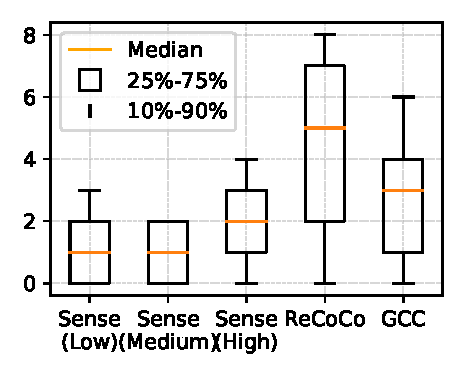
\includegraphics[width=\linewidth]{figures/chap03/evaluation_plots/jitter_times.pdf}
  \caption{抖动次数}
  \label{fig-jitter-times}
\end{subfigure}

\caption{训练及运行性能}
\label{fig-evaluation-result}
\end{figure}

            \end{block}
    
            \end{column}
    
            \begin{column}{0.5\textwidth}
            \begin{colorblock}[black]{sinteflightgreen}{}
                % Please add the following required packages to your document preamble:
% \usepackage{booktabs}
% \usepackage{multirow}
\begin{table}[ht]
\caption{Sense的QoE实验结果与其他方法对比}
\vspace{-0.5em}
\renewcommand{\arraystretch}{0.8} % 调整竖直方向的行高
\resizebox{\linewidth}{!}{%
\begin{tabular}{@{}cccccccccc@{}}
\toprule
网络条件 & 游戏类型分类 & 方法 & 平均延迟 & 尾部延迟 (95\%) & 平均 r($L_{MTP}$) & 平均发送速率(Kbps) & $R_slog(s)$ & 抖动次数 & 最终 QoE \\ \midrule
\multirow{9}{*}{\begin{tabular}[c]{@{}c@{}}高吞吐量\\      ($\geq$ 10Mbps)\end{tabular}} & \multirow{3}{*}{高敏感度} & ReCoCo               & 50.501          & 101.166             & 2.802             & 4748.340               & 4.610    & 6            & 1.728          \\
                                                                                                      &                            & GCC                  & 53.776          & 130.871             & 2.563             & 1926.600               & 3.935    & 3            & 1.687          \\
                                                                                                      &                            & \textbf{Sense(提出方法)} & 50.600          & 102.690             & 2.794             & 4379.535               & 4.549    & 3            & \textbf{1.898} \\ \cmidrule(l){2-10} 
                                                                                                      & \multirow{3}{*}{中敏感度}    & ReCoCo               & 50.501          & 101.166             & 3.739             & 4748.340               & 4.610    & 6            & 1.962          \\
                                                                                                      &                            & GCC                  & 53.776          & 130.871             & 3.621             & 1926.600               & 3.935    & 3            & 1.952          \\
                                                                                                      &                            & \textbf{Sense(提出方法)} & 50.600          & 101.000             & 3.736             & 2795.595               & 4.214    & 1            & \textbf{2.175} \\ \cmidrule(l){2-10} 
                                                                                                      & \multirow{3}{*}{低敏感度}       & ReCoCo               & 50.501          & 101.166             & 4.424             & 4748.340               & 4.610    & 6            & 2.133          \\
                                                                                                      &                            & GCC                  & 53.776          & 130.871             & 4.292             & 1926.600               & 3.935    & 3            & 2.119          \\
                                                                                                      &                            & \textbf{Sense(提出方法)} & 51.726          & 105.333             & 4.376             & 4582.741               & 4.583    & 0            & \textbf{2.490} \\ \midrule
\multirow{9}{*}{\begin{tabular}[c]{@{}c@{}}低吞吐量\\      (\textless 10Mbps)\end{tabular}}     & \multirow{3}{*}{高敏感度} & \textbf{ReCoCo}      & 53.771          & 110.143             & 2.563             & 237.945                & 2.371    & 4            & \textbf{1.234}          \\
                                                                                                      &                            & GCC                  & 177.772         & 1277.680            & 1.000             & 186.950                & 2.190    & 2            & 0.923          \\
                                                                                                      &                            & Sense(提出方法)          & 66.761          & 210.250             & 1.720             & 277.849                & 2.487    & 3            & 1.114          \\ \cmidrule(l){2-10} 
                                                                                                      & \multirow{3}{*}{中敏感度}    & ReCoCo               & 53.771          & 110.143             & 3.622             & 237.945                & 2.371    & 4            & 1.498          \\
                                                                                                      &                            & GCC                  & 177.772         & 1277.680            & 1.000             & 186.950                & 2.190    & 2            & 0.923          \\
                                                                                                      &                            & \textbf{Sense(提出方法)} & 60.397          & 111.000             & 3.373             & 271.060                & 2.468    & 2            & \textbf{1.585} \\ \cmidrule(l){2-10} 
                                                                                                      & \multirow{3}{*}{低敏感度}       & \textbf{ReCoCo}      & 53.771          & 110.143             & 4.292             & 237.945                & 2.371    & 4            & \textbf{1.666}          \\
                                                                                                      &                            & GCC                  & 177.772         & 1277.680            & 1.000             & 186.950                & 2.190    & 2            & 0.923          \\
                                                                                                      &                            & Sense(提出方法)          & 67.640          & 220.200             & 3.533             & 230.204                & 2.346    & 2            & 1.595          \\ \bottomrule
\end{tabular}
}
    \label{tab:exp_results}
\end{table}
            
            \end{colorblock}
            
            \begin{colorblock}[black]{sintefyellow}{}
                                \begin{table}[ht]
            \centering
            \caption{敏感度误分类对QoE的影响}
            \renewcommand\arraystretch{1.25}
            \resizebox{0.9\columnwidth}{!}{%
            \begin{tabular}{@{}cccc@{}}
            \toprule
            \textbf{案例} & \textbf{QoE} & \textbf{相较于正确分类的 QoE} & \textbf{相较于最低基准的 QoE} \\ \midrule
            应为高敏感度但被误分类为低敏感度 & 1.84  & -7.43\%                     & +0.54\%                     \\ 
            应为低敏感度但被误分类为高敏感度 & 2.30  & -0.90\%                     & -0.04\%                     \\ \bottomrule
            \end{tabular}
            }
            \label{miscals}
            \end{table}
            \end{colorblock}

        \end{column}
    \end{columns}
\end{frame}
\section{基于预训练大模型的网络控制策略选择范式设计}

\begin{frame}[fragile]{基于预训练大模型的网络控制策略选择范式设计}
\framesubtitle{设计动机}
% 请将以下所需的宏包添加到文档前言:
% \usepackage{booktabs}
% \usepackage{multirow}
\begin{table}[ht]
\caption{各种任务中使用的经典算法}
\resizebox{0.6\textwidth}{!}{ % 调整表格宽度以适应页面

\begin{tabular}{@{}ccccc@{}}
\toprule
\textbf{任务}                                          & \textbf{目标}                                 & \textbf{策略}      & \textbf{原理}        & \textbf{年份} \\ \midrule
\multirow{6}{*}{\textbf{自适应码率}}            & \multirow{6}{*}{重缓冲、比特率、比特率变化}   & Pensieve           & 基于强化学习        & 2017          \\
                                                       &                                              & Genet             & 基于强化学习        & 2022          \\
                                                       &                                              & MPC               & 动态规划            & 2015          \\
                                                       &                                              & BBA               & 基于缓冲区          & 2014          \\
                                                       &                                              & BOLA              & 基于缓冲区          & 2016          \\
                                                       &                                              & NetLLM            & 基于Transformer     & 2024          \\ \midrule
\multirow{6}{*}{\textbf{拥塞控制}}                      & \multirow{6}{*}{吞吐量、丢包、延迟}           & CUBIC             & 基于丢包            & 1990年代       \\
                                                       &                                              & Reno              & 基于丢包            & 1990年代       \\
                                                       &                                              & WestWood          & 基于丢包            & 2002          \\
                                                       &                                              & BBR               & 基于带宽-延迟积     & 2015          \\
                                                       &                                              & Aurora            & 基于强化学习        & 2019          \\
                                                       &                                              & Sage              & 基于强化学习        & 2023          \\ \bottomrule
\end{tabular}
}
\label{table_task_algo}
\end{table}

\begin{itemize}
    \item 单一算法性能的局限性构成不同的网络环境和需求下的次优。
\end{itemize}

\end{frame}

\begin{frame}[fragile]{基于预训练大模型的网络控制策略选择范式设计}
\framesubtitle{设计动机}
\begin{figure}
    \centering
    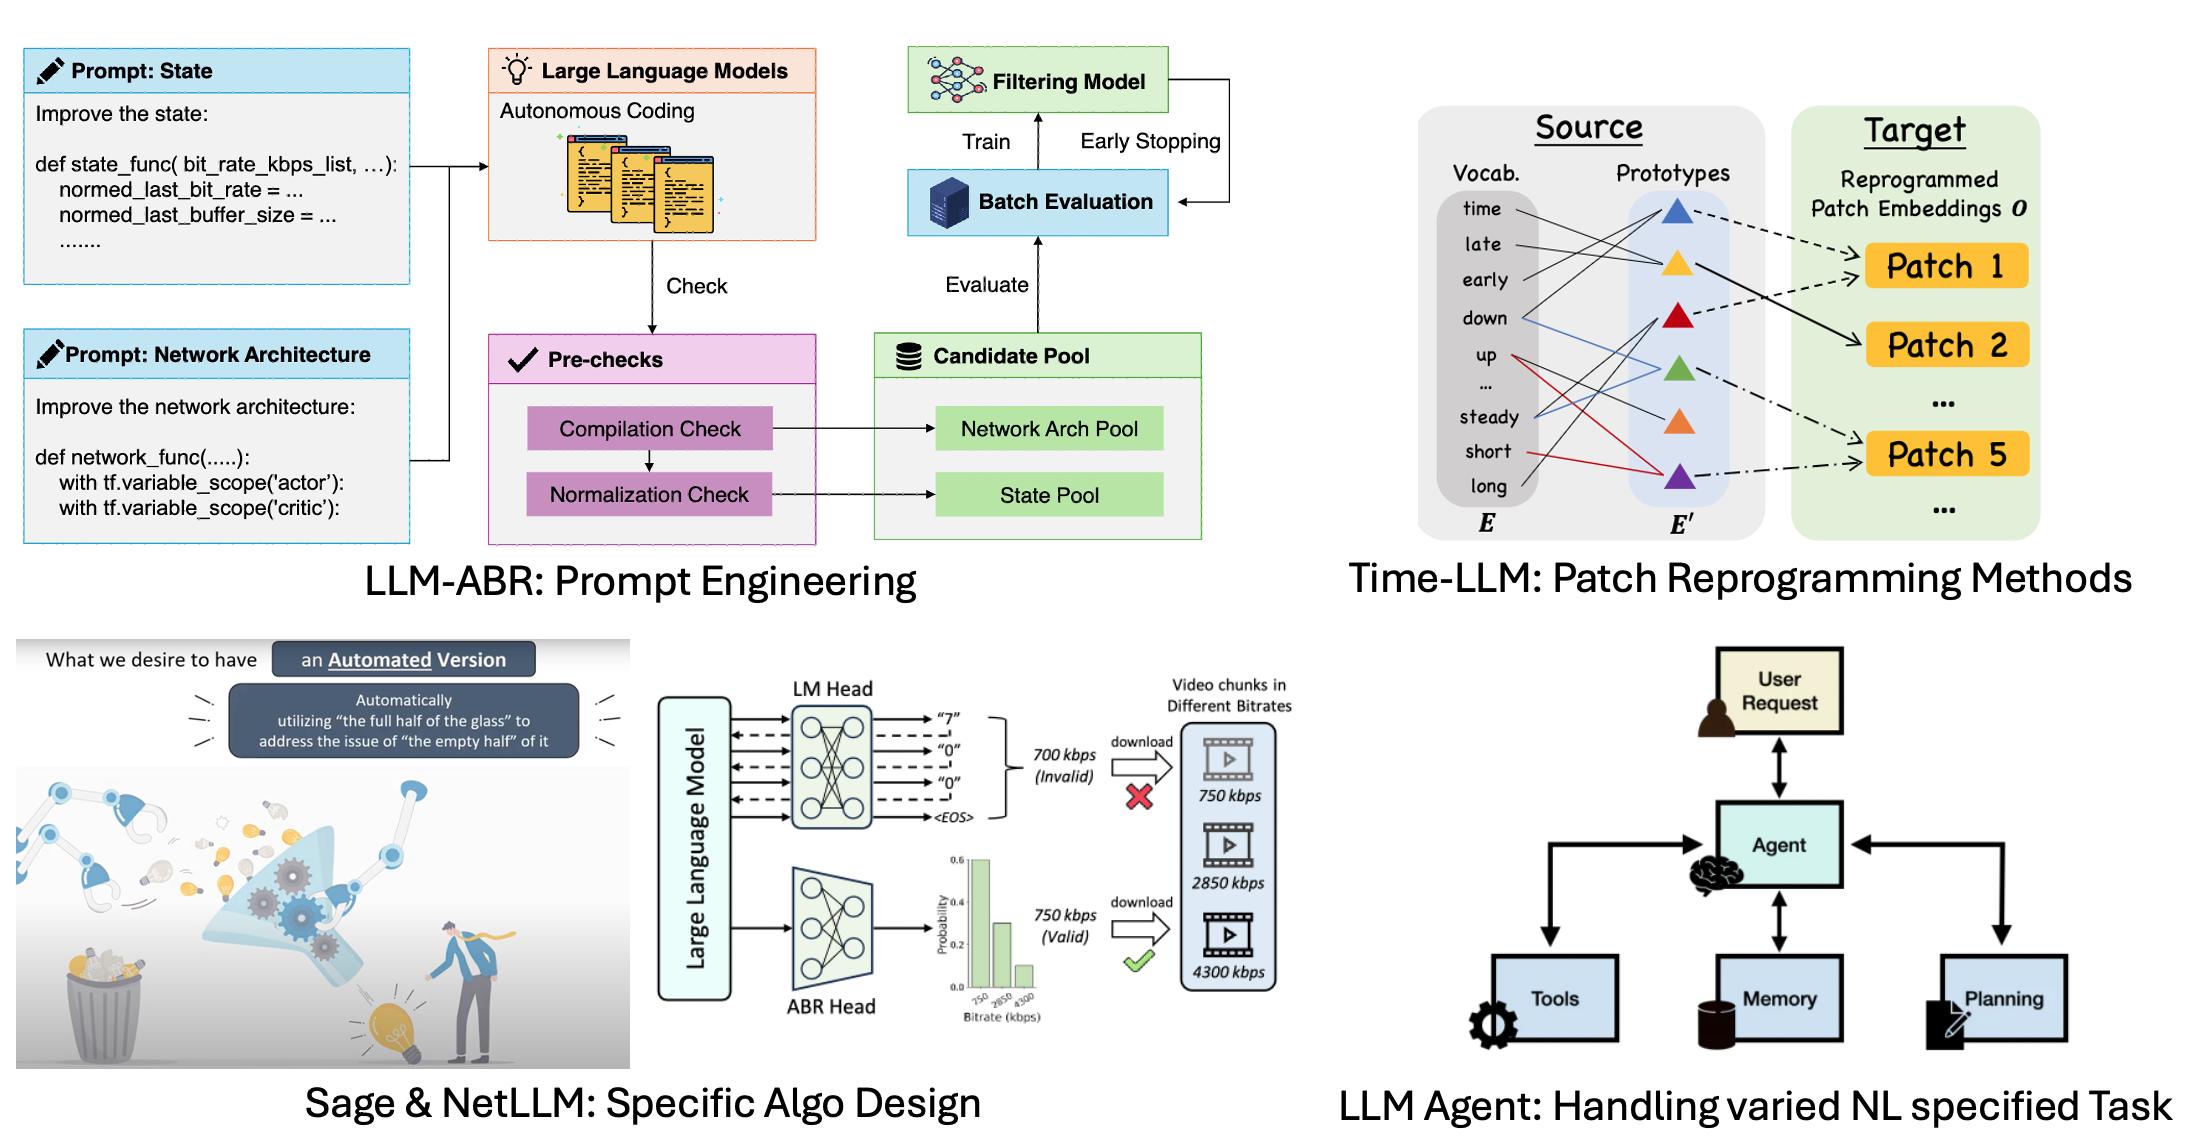
\includegraphics[width=0.6\linewidth]{figures/截屏2024-12-02 16.28.42.png}
    \caption{大模型的能力与应用}
    \label{fig:enter-label}
\end{figure}
\begin{itemize}
    \item 大语言模型在环境感知理解、规划和决策方面具有强大的能力,表明它们具有感知网络环境、理解应用需求并做出相应规划的潜力。
\end{itemize}


\end{frame}


\begin{frame}[fragile]{基于预训练大模型的网络控制策略选择范式设计}
\framesubtitle{设计方案构思}

\begin{figure} [ht]
\centering
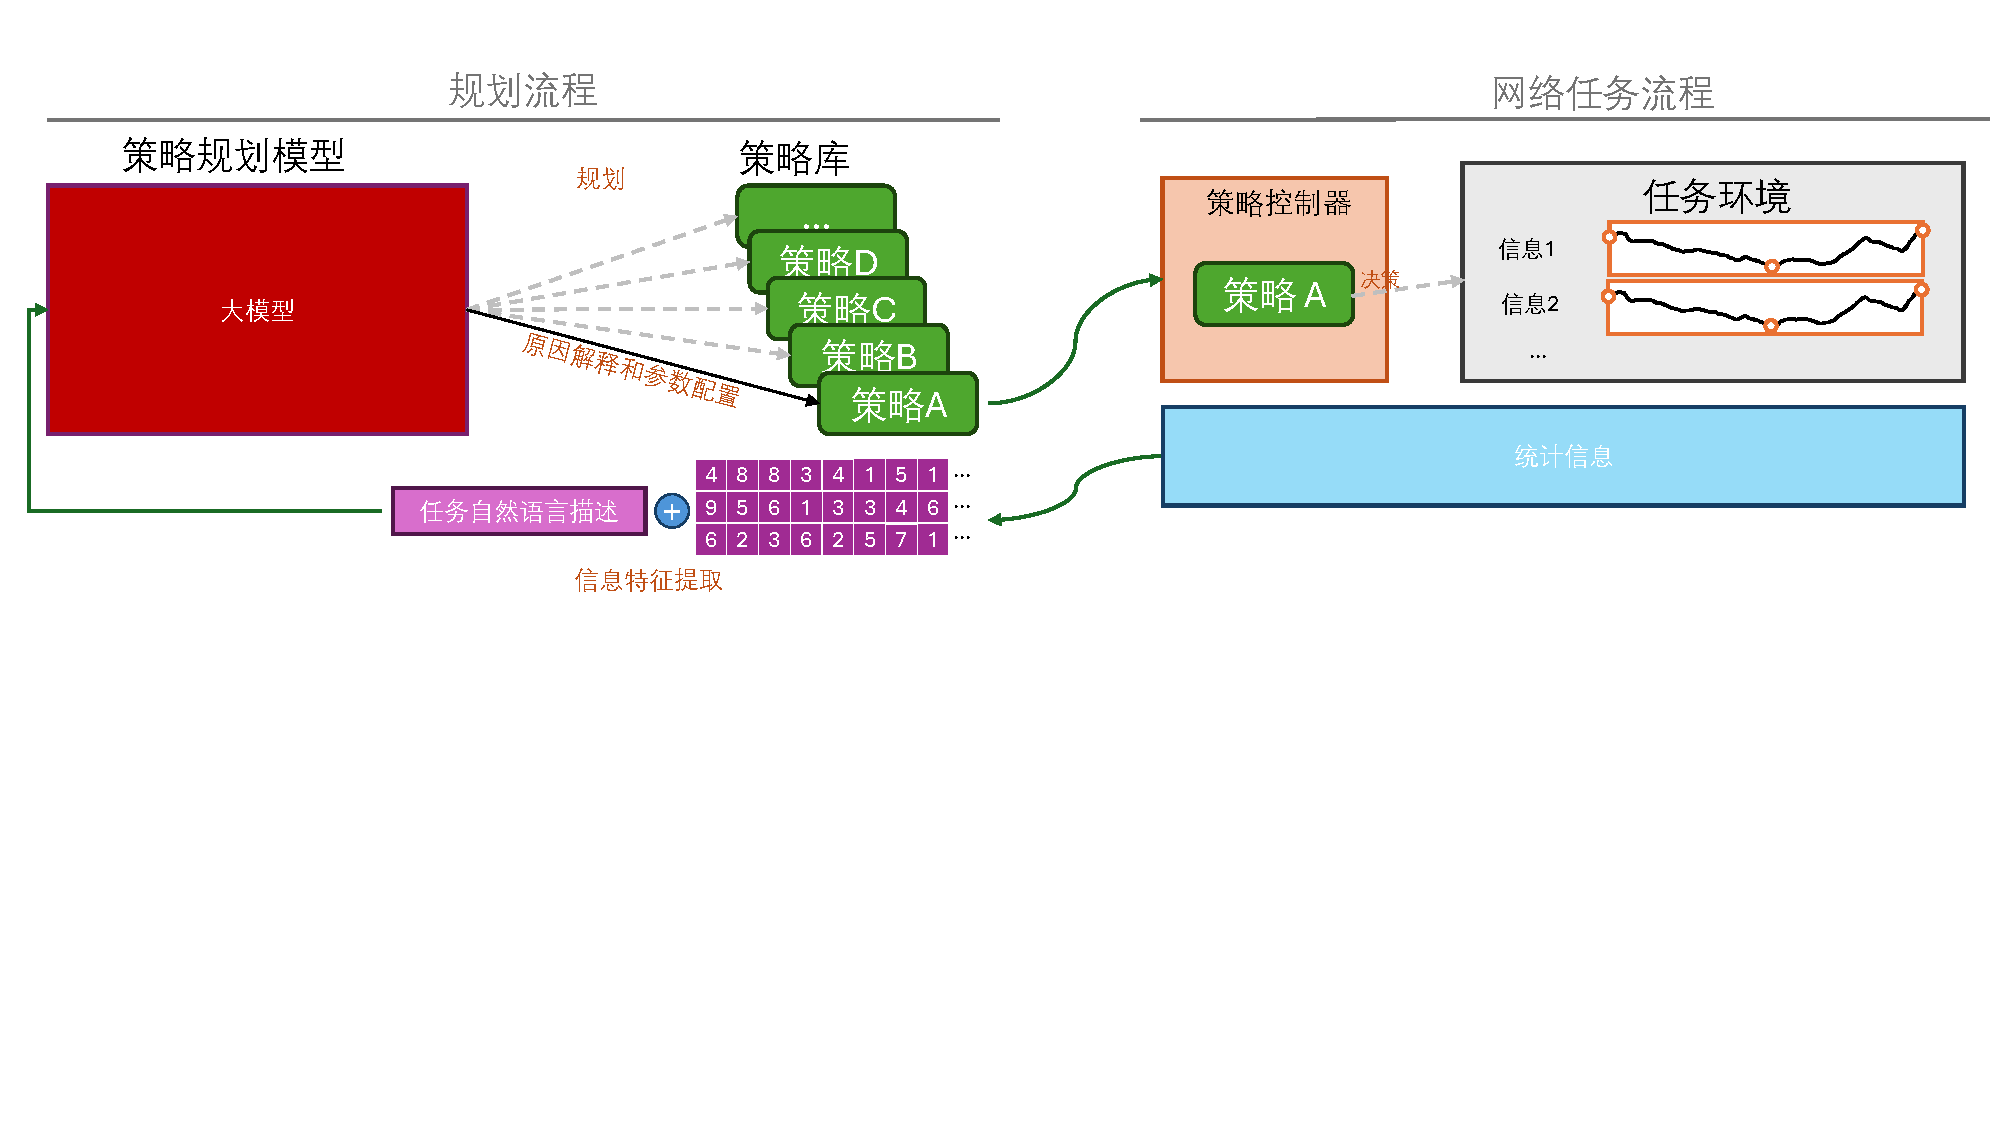
\includegraphics[width=\textwidth]{figures/作图.pdf} 
\caption{网络控制策略选择范式设计概览}
\label{fig_llmcc_design}
\end{figure}
\begin{itemize}
    \item 可利用大模型构建新范式,在该范式中,基于网络状况,预训练的 LLM 从策略库中选择“最适合的”策略,从而实现动态的宏观策略切换,增强算法选择的适应性。
\end{itemize}
\end{frame}




\begin{frame}[fragile]{基于预训练大模型的网络控制策略选择范式设计}
\framesubtitle{设计方案构思}
\begin{figure}
    \centering
    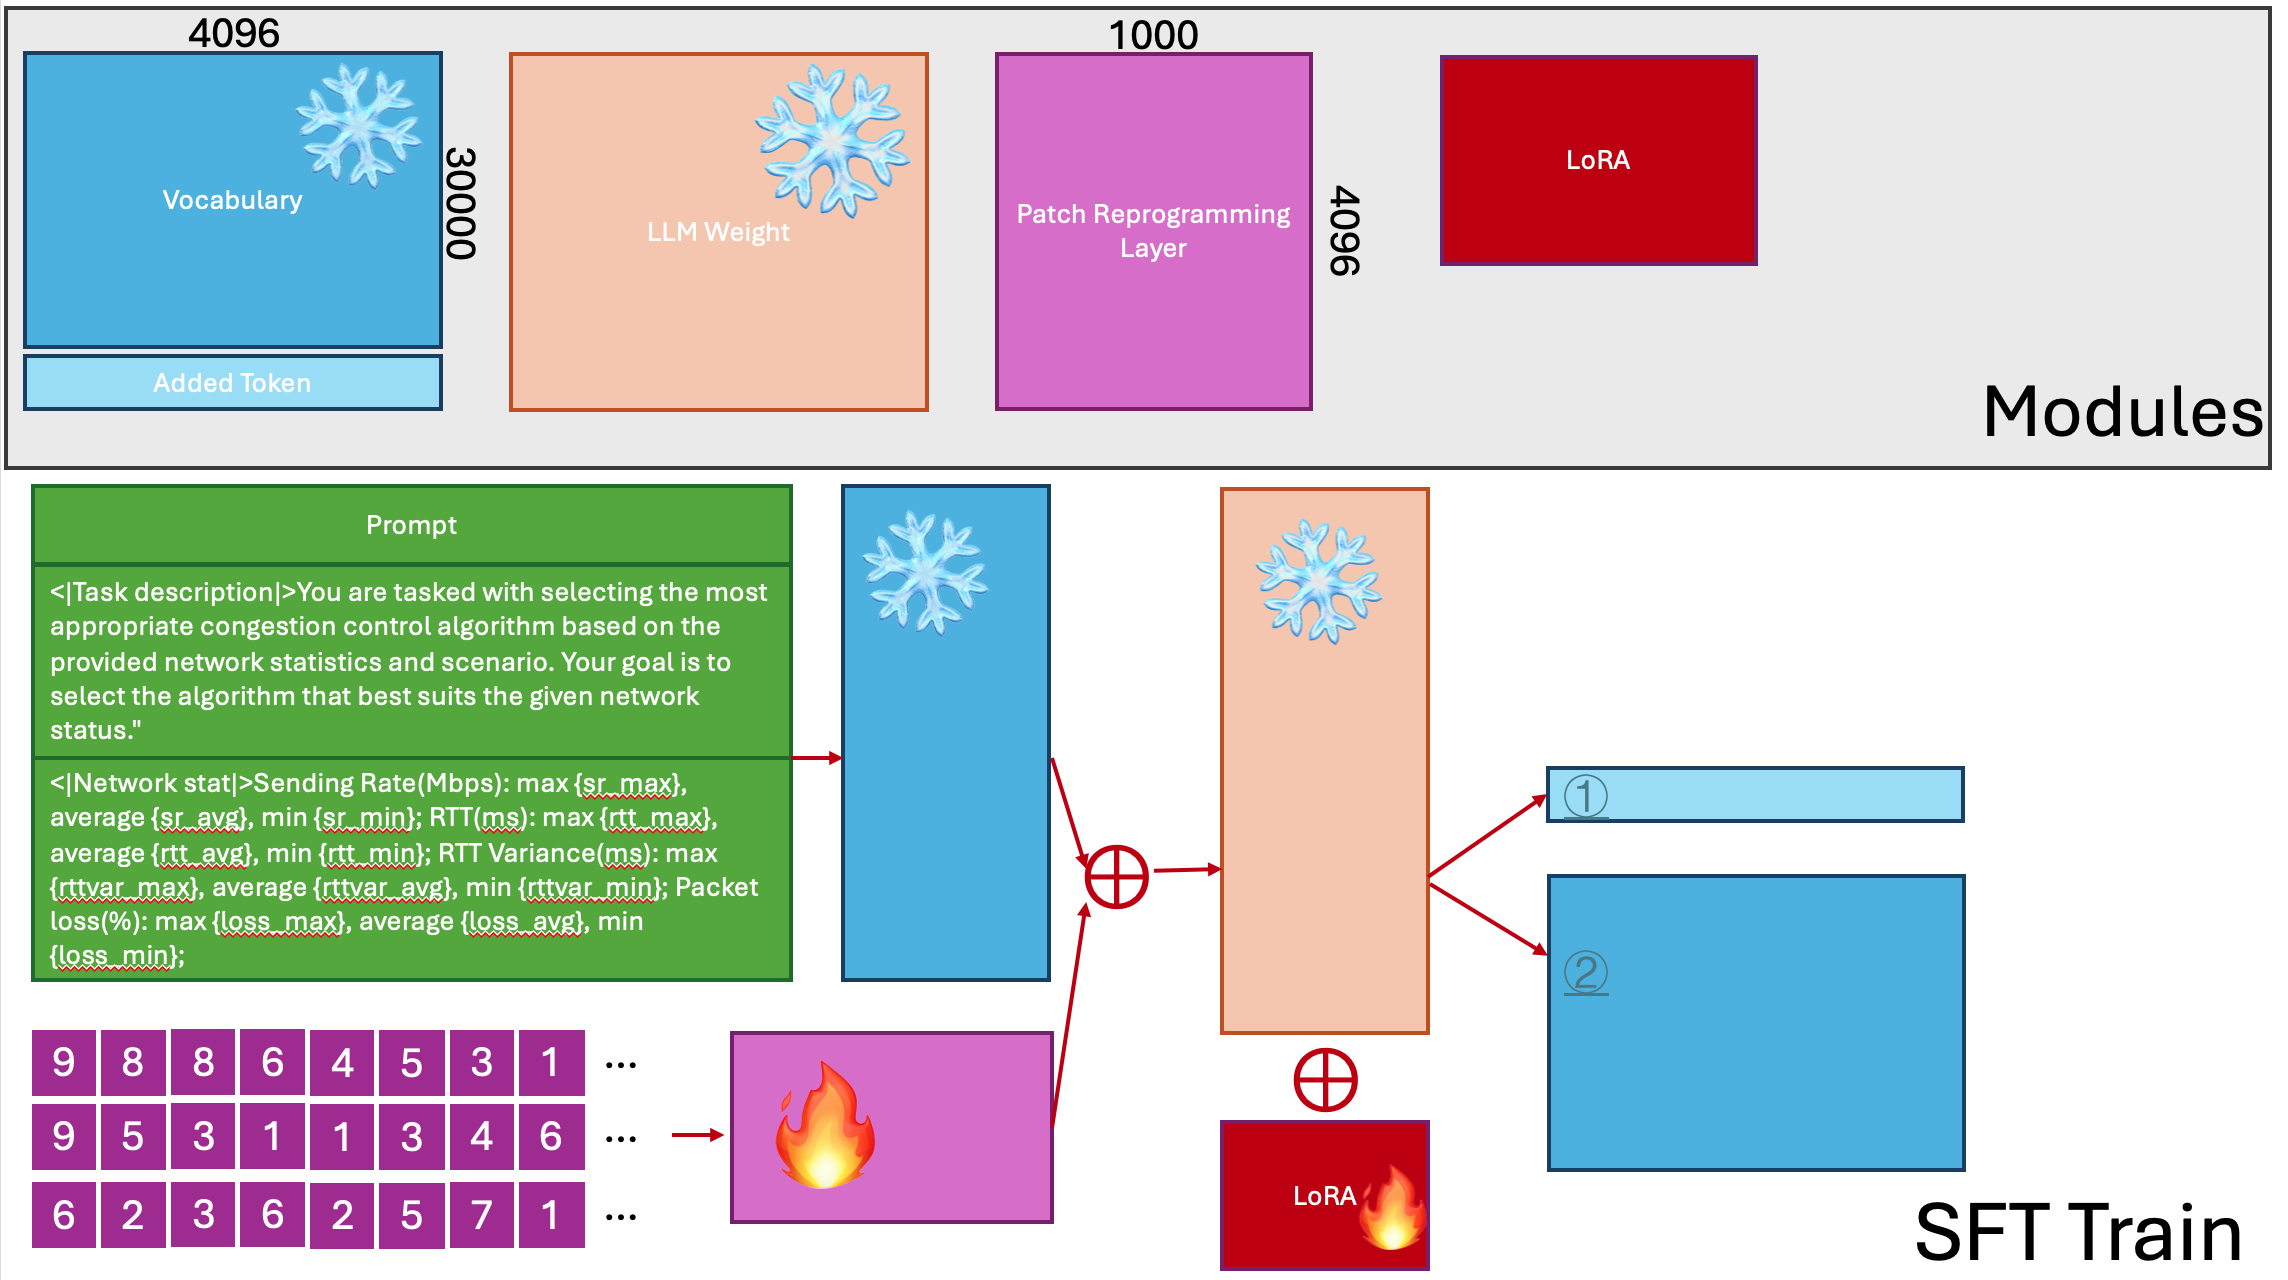
\includegraphics[width=0.75\linewidth]{figures/截屏2024-12-02 16.31.42.png}
    \caption{大模型的模块和微调权重概览}
    \label{fig:enter-label}
\end{figure}

\end{frame}

\section{研究计划与进展}
\begin{frame}[fragile]{研究计划与进展}
\begin{table}[ht]
    \caption{研究计划表}
    \renewcommand\arraystretch{1.25}
    \centering
    \resizebox{0.6\columnwidth}{!}{%
    \begin{tabular}{@{}cc@{}}
\toprule
时间 & 安排                                                           \\ \midrule
2024.12     & 完善网络控制策略选择范式设计的实验                          \\
2025.01     & 撰写网络控制策略选择范式设计的论文,投稿                   \\
2025.03     & 总结工作,完成毕业论文        \\            \bottomrule
\end{tabular}
    }
    \label{tab:agrnksd}
\end{table}
    

\end{frame}

\begin{frame}[fragile]{研究计划与进展}
\begin{itemize}

\item \textbf{Xuanyu Zhu}, Shuzhao Xie, Zhi Wang.Sense: Latency Sensitivity-Aware RL Rate Control for Cloud Gaming[C]. Proceedings of the AAAI Conference on Artificial Intelligence. (CCF-A, under review)
    
    \item \textbf{Xuanyu Zhu}, Duo Wu, Wei Zhang, Zhi Wang. Network Task Policy Selection Based on Large Language Models[C]. Proceedings of the ACM SIGCOMM 2025 Conference. (CCF-A, in preparation)
    
    \item Shiqi Dai, \textbf{Xuanyu Zhu}, Naiqi Li, Zhi Wang. Procedural level generation with diffusion models from a single example[C]. Proceedings of the AAAI Conference on Artificial Intelligence. 2024, 38(9): 10021-10029. (CCF-A)
\end{itemize}
\end{frame}
\footlinecolor{sintefyellow}
\backmatter




\begin{frame}[allowframebreaks]{参考文献}
\framesubtitle{参考文献}

    \begin{itemize}[noitemsep]  % 禁止项目符号的间距
            \footnotesize  % 设置局部字体大小
            \printbibliography[heading=none]  % 输出参考文献
    \end{itemize}
\end{frame}




\end{document}
